\label{sec:field}

The steady virtual vane model was used to explore a broad set of
system configurations to optimize the system turning vane
configuration to maximize the kinetic energy flux into the facility. 
Based on the lessons learned in Chapter~\ref{sec:results}, as
well an extensive optimization effort, a new configuration was created
and explored computationally. The resulting configuration represents a
significant change from that used in the August 2015 Field test. This
chapter begins by describing the geometry of the device and the design
optimization that lead to this configuration. Next is a detailed look
at the turbine design incorporated into the SoV to extract energy from
the flow. A field prediction based on the computational model is
then provided. Some of the model shortcomings of this design are
considered, with corrections for the model deficiencies proposed and the
results of these corrections to the baseline models explored. Finally,
the chapter concludes with an estimate of the maximum energy that could
be extracted from an idealized turbine placed within this device.   

\section{System Geometry}

The new field geometry represents a significant departure from
the August 2015 system, which was designed largely by the experimental
team at Georgia Tech. Computer Aided Design (CAD) images of the 2015
system from the top and side are shown in Figure~\ref{fig:cad_aug_2015},
albeit without the cone. An actual image of the 2015 field configuration
is in Figure~\ref{fig:aug_2015_field}. The inner diameter of the second
tier vanes for this apparatus was six meters, and the overall vane
height was nearly three meters. The second tier vanes were straight and
constructed from fiberglass. The sixty minute time averaged integral
of the kinetic energy flux was measured at 107 Watts, but demonstrated
large variations, with an RMS of 79.4 Watts and a peak power of 784
Watts. The peak power corresponds to periods with the largest ambient
wind velocities, and this is considered an indicator of the 
importance of the wind in the newly proposed asymmetric design.  

%
% 51 degrees top
%The upper tier was set at 51 degrees (relative to the radial direction)
%from the pivot. 
%
% 
% The lower tier vanes were 75 degrees away from the radial inward
% direction or 15 degrees from azimuthal.  


  \begin{figure}
   \centering
   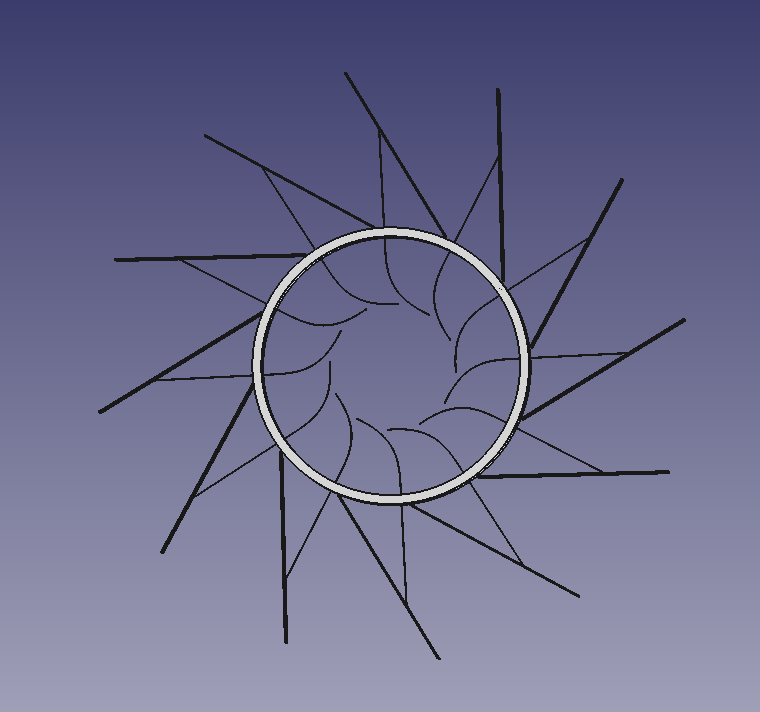
\includegraphics[width =0.4\textwidth]{figs/aug_test_top}
   \hfill
   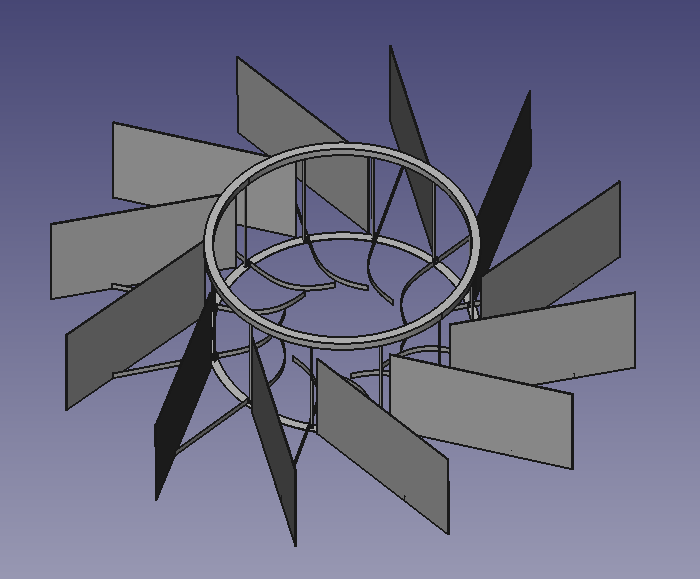
\includegraphics[width =0.45\textwidth]{figs/aug_test_side}
   \caption{August 2015 Field Test CAD images. An image from the top
   down is on the left, and an angled view on the right. Both images do
   not include the cone. The CAD designs were created by the team at
   Georgia Tech. The images were created from these CAD files by the
   author using FreeCAD\cite{Falck}.}  
   \label{fig:cad_aug_2015}
  \end{figure}

Starting from this baseline, and armed with the steady virtual vane
model, an extensive design effort was embarked upon to explore a large space
of possible system configurations and geometries to develop a new 
SoV apparatus. To arrive at the present design, the
process also included weekly calls with the experimental team to discuss
possible system designs.  

This conceptual phase generated a wide range of possible
configurations, few of which showed enough promise to warrant further
investigation. The designs that produced initially promising results were
then optimized as outlined in 
Section~\ref{sec:results}, where new parameter values were specified, a
simulation was performed, and then the output was postprocessed to evaluate the
energy flux. In this way several
hundred optimization runs were performed over the course of several
months. While not provably exhaustive, this extensive exploration of the 
SoV configuration space covered the major design concepts detailed
in Section~\ref{sec:dust_devil_concept}. 

  \begin{figure}
   \centering
   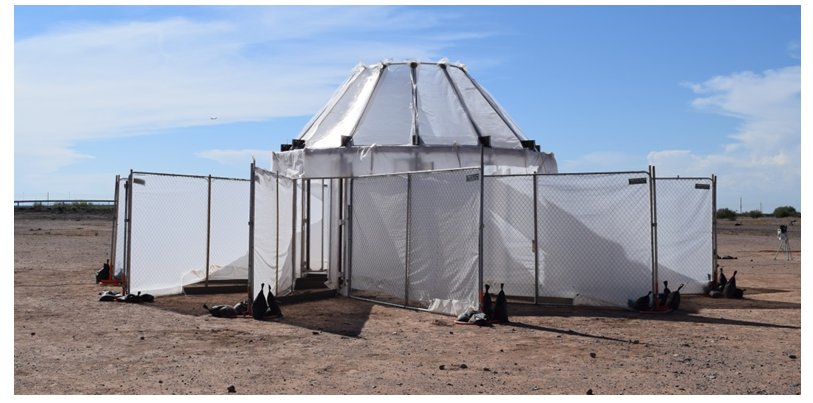
\includegraphics[width =0.7\textwidth]{figs/aug_2015_field}
   \caption{A photo of the August 2015 Field Configuration. Image
   credit: Dr. Mark Simpson.}  
   \label{fig:aug_2015_field}
  \end{figure}

The new configuration is highly asymmetric, which is intended to capture
the wind over 
a much greater area and draw it into the
device. Horizontal and vertical views of the new optimized configuration
are shown in Figures~\ref{fig:top_design},\ref{fig:bottom_design} and
\ref{fig:vertical_design}, below. The parameters describing the
vanes are detailed in Tables~\ref{tab:top},\ref{tab:bottom} and
\ref{tab:side}. This design does have some notable 
similarities to the previous iterations. It retains the two-tier
design outlined Section~\ref{sec:dust_devil_concept}. The inner diameter 
of the 2\textsuperscript{nd} tier vanes remains six meters, and the
bottom tier is much shorter than the second tier. A brief summary of the
differences are provided below:      

\begin{itemize}
\item The bottom tier vanes are taller than in the previous field test, 
      and their height is asymmetric, with taller vanes on the down-wind side
\item An impermeable cylinder was introduced along the arc $\{\pi < \theta
      < 0 \}$, e.g. the bottom two quadrants in the images below, replacing the
vanes in those quadrants. 
\item The upper tier vanes were configured to align with the freestream
velocity, to provide a larger wind-driven flux into the facility.
\item Horizontal partitions were added to the top of the upper vanes, to
prevent flow in the vanes from rising up and out of the vanes
\item The cone is taller providing a greater contraction
\end{itemize}

We now discuss each of these changes in detail. Simulations indicated that 
the
bottom tier vanes were too short, and were constricting the flow 
through them. Originally, the height of the lower
tier vanes was set based on the thickness of the 
thermal boundary layer, but the original boundary layer inside
the vanes was considerably thicker than measurements indicated. 
This is presumed to be a result of the
convection of ground-heated air into the device by ambient winds and
the strong radial entrainment by the vortex. If true, then a shorter
first tier is a substantial impediment to the intensification of the
vortex, as it limits the inflow of heated air which, as detailed
in Section\ref{sec:wind_impact}, probably plays an important role in 
the operation of the device.

The downwind side lower tier vanes are, by a factor of two, taller 
than the upwind side. This
is because the downwind boundary layer is thicker due to its 
lower Reynolds number. The Reynolds number is lower on the
downwind side because it is not being driven by the wind.
For this reason, the downwind lower tier
vanes also have a lower maximum turning angle to reduce blockage.

Despite repeated efforts, the downwind side of the second tier vanes were
never found to entrain flow from the wake, even with the vane separation
model detailed in Section~\ref{sec:separation}. As ``leakage'' of the
vortex out the back of the SoV has been a noted issue in the past, it
was decided to introduce an impermeable cylindrical wall along the
regions where leakage was observed to occur in the simulations. 

The most visually striking change between the current configuration and
the previous field configuration is in the second tier vanes. 
Since the wind was found to be a
significant fraction of the energy flux entering the device , 
 the upper tier vanes were redesigned to capture as much of this
energy as possible. To do this, the vanes were extended far out in the
streamwise direction and aligned with the freestream velocity. 
This broken symmetry introduces a failure mode, as it
requires that the facility be aligned with the streamwise velocity, which of 
course can change. This design decision is discussed in more detail in
Section~\ref{subsec:scenario_param}. 

The upper tier vanes also now possess horizontal partitions. By placing
a flat horizontal ``top'' on the vanes, flow is constrained from
leaving the SoV apparatus before it is forced into the
center. This horizontal partition is clearly visible in
Figure~\ref{fig:top_down_cad}.   

The cone plays at least two important roles. The first is acting as a
converging nozzle for the flow, increasing the vertical and azimuthal
velocity as it exits out the top of the device. Additionally, much like
a wind tunnel contraction, the cone increases the
symmetry of the flow near the exit. This is important because the turbine 
can more easily extract power from a symmetric velocity
field. 
Second, the cone also acts as a shield, preventing the wind
from disrupting the vortex before it has run through the
turbine. A taller cone than had been previously used was found 
to be more effective in both of these ways.

It is important to note that while increasing the height of the cone
(and along with it, the contraction ratio) was recommended, due to
time and fabrication constraints this particular cone design was not
implemented. The cone design quoted below was the cone used by
the field team, despite being found to be sub-optimal in
simulations. All the simulations shown in this chapter are consistent
with the design used in the 2016 field tests, and this unrealized cone
optimization is noted for completeness.

 \begin{figure}[!htb]
  \begin{center}
   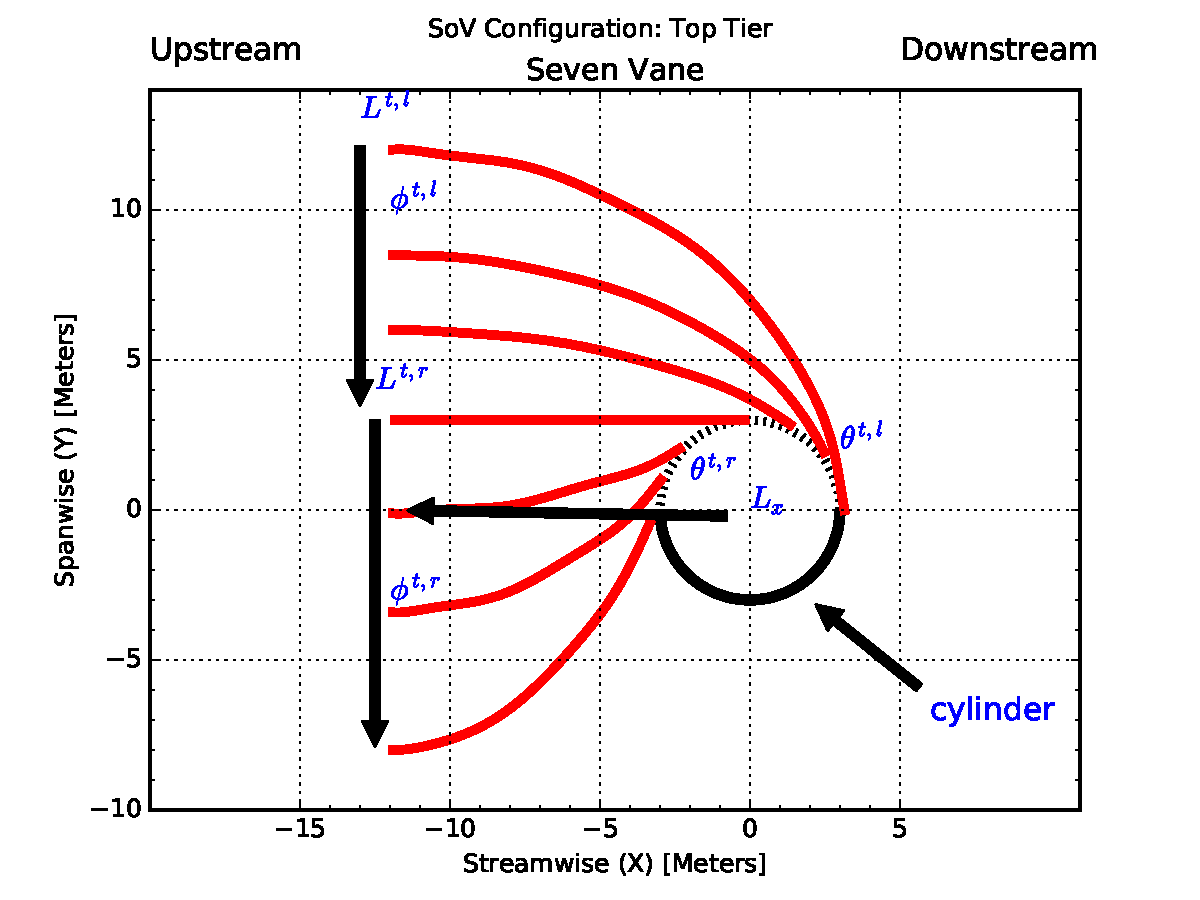
\includegraphics[width =0.7\textwidth]{figs/interp_entire_top.pdf}
   \caption{A top view of the top vane design. The red lines are the
     vanes, which are spaced so that the mass flux between vanes is
     approximately equal. The blue symbols are the parameters that
     specify the design. Notice the highly asymmetric configuration,
     with the front (left) opening of the vanes aligned directly with
     the incoming wind. Also note the slight ``wiggle'' in the second
   vane from the bottom. This is a result of the polynomial
   interpolation function used to generate the vanes, which is described
   in Section~\ref{sec:interpolate}.} 
   \label{fig:top_design}
  \end{center}
 \end{figure}

\begin{table}[]
\centering
 \caption{The parameters used in the top tier system
 geometry. Parameters labeled with $\phi$ are angles relative to
 streamwise direction ($\hat i$), while the $\theta$ parameters are
 angles relative to radial direction ($\hat r$). $\alpha$ is the angle
 from origin to inner terminus of vane, and so in this way some vane
 angles are smoothly varying as a function of polar angle. See
 Figure~\ref{fig:top_design} for a schematic depicting the vanes. The
 superscript $t$ denotes top, or the second tier vanes. Among the top
 tier vanes, $l$ is left, $r$ right (when viewed from upstream of the
 device).}
\begin{tabular}{l|l|l}
Name                        & Value & Meaning                    \\
 \hline
$r^{\text{cyl}}$            &  3.0 meters & Radius of rigid cylinder \\
$r^t_{\text{min}}$          &  3.0 meters & Smallest radius of top tier
	 vanes, relative to ground \\
$L_x$                       &  12 meters  & Distance upstream
	 of vanes relative to center\\
$\phi^{t,l}$ &  $0^{\circ}$   & Outer angle for the top tier, left side vanes \\
$\phi^{t,r}$   &  $0^{\circ}$   & Outer angle for the top tier right side \\
$\theta^{t,l}$ &   $30^{\circ} +\frac{\alpha}{3}$  & Inner angle for the top tier left side vanes\\
$\theta^{t,r}$   &   $75^{\circ} +\frac{\alpha}{6}$   & Inner angle for the top tier right side \\
$L^{t,r}$                   &  12 meters  & Width of vane in front of cylinder \\
$L^{t,l}$                   &  10 meters  & Width of vane to the side of cylinder \\
\end{tabular}
 \label{tab:top}
\end{table}

%The values of the parameters depicted in
%Tables~\ref{tab:top},\ref{tab:bottom} and \ref{tab:side} bear some
%discussion. 

% Forcing function has a discontinuity at $\alpha=90^{\circ}$

 \begin{figure}[!htb]
  \begin{center}
   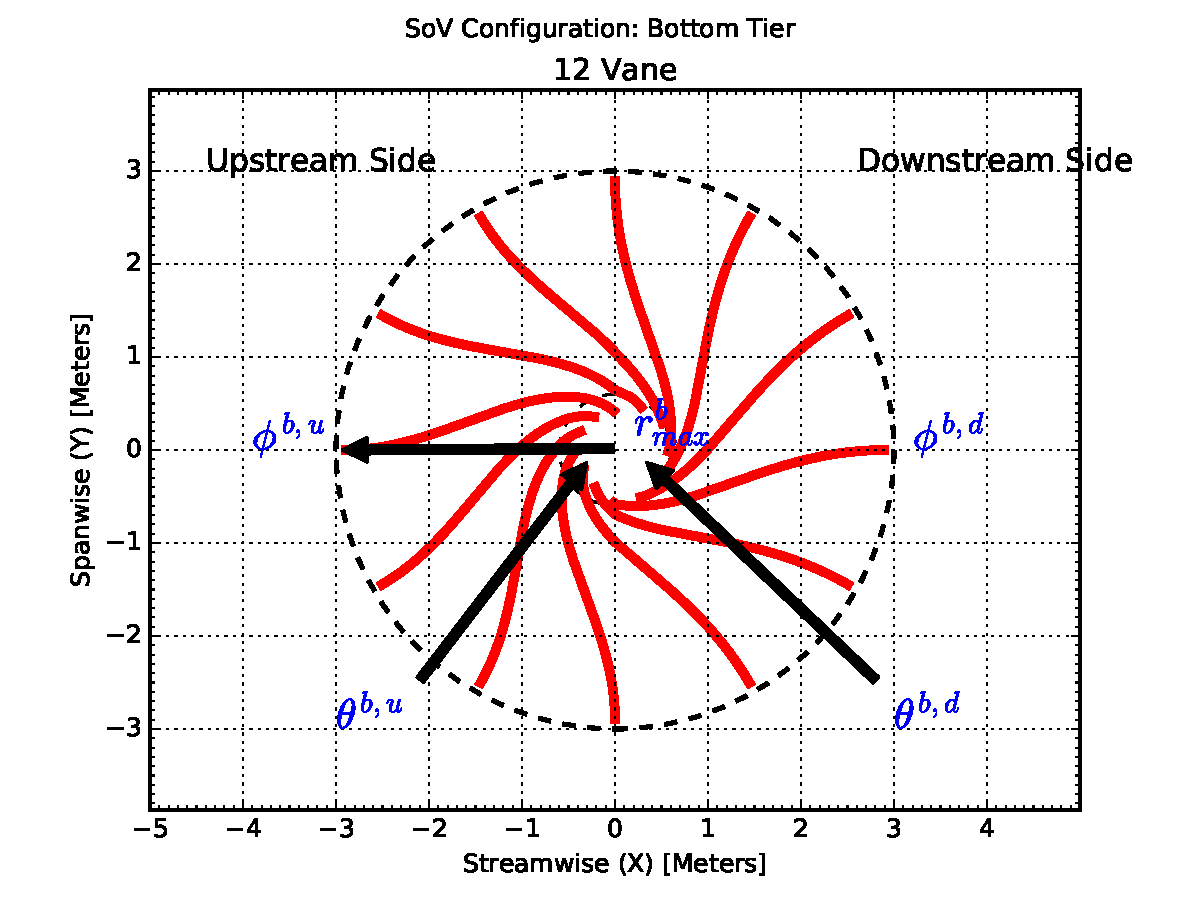
\includegraphics[width =0.7\textwidth]{figs/interp_entire_bottom.pdf}
   \caption{A top view of the bottom tier design. These vanes (in red)
   are also asymmetric, with lower final curvature angles and a taller
   height for the back (downstream) vanes versus the front. This is due
   to the thicker boundary layer of the flow entering the device from
   the right (downstream relative to the wind). These vanes are design
   to turn the incoming flow so that it is nearly azimuthal near the
   center of the apparatus, increasing rotation and lowering the
   pressure in the center.}
   \label{fig:bottom_design}
  \end{center}
 \end{figure}

\begin{table}[]
\centering
 \caption{The parameters used in the bottom tier system geometry. See 
 Figure~\ref{fig:bottom_design} for a schematic depicting these
 vanes. The superscript $b$ denotes bottom tier, $d$ is downstream, $u$
 for upstream vanes. In this case, both $\phi$ and $\theta$ are angles
 relative to radial ($\hat r$). }
\begin{tabular}{l|l|l}
Name                        & Value & Meaning                    \\
 \hline
$r^b_{\text{min}}$          &  0.6 meters & Smallest radius of bottom tier vanes \\
$r^b_{\text{max}}$          &  6.0 meters & Largest radius of bottom tier vanes \\
$\theta^{b,d}$ &  $60^{\circ}$   & Inner angle for the bottom tier, downstream vanes \\
$\theta^{b,u}$ &  $80^{\circ}$   & Inner angle for the bottom tier, upstream vanes \\
$\phi^{b,d}$ &   0   & Outer angle for the bottom  tier, downstream vanes \\
$\phi^{b,u}$ &   0   & Outer angle for the bottom tier, upstream vanes \\
\end{tabular}
 \label{tab:bottom}
\end{table}


\begin{figure}[!htb]
  \begin{center}
   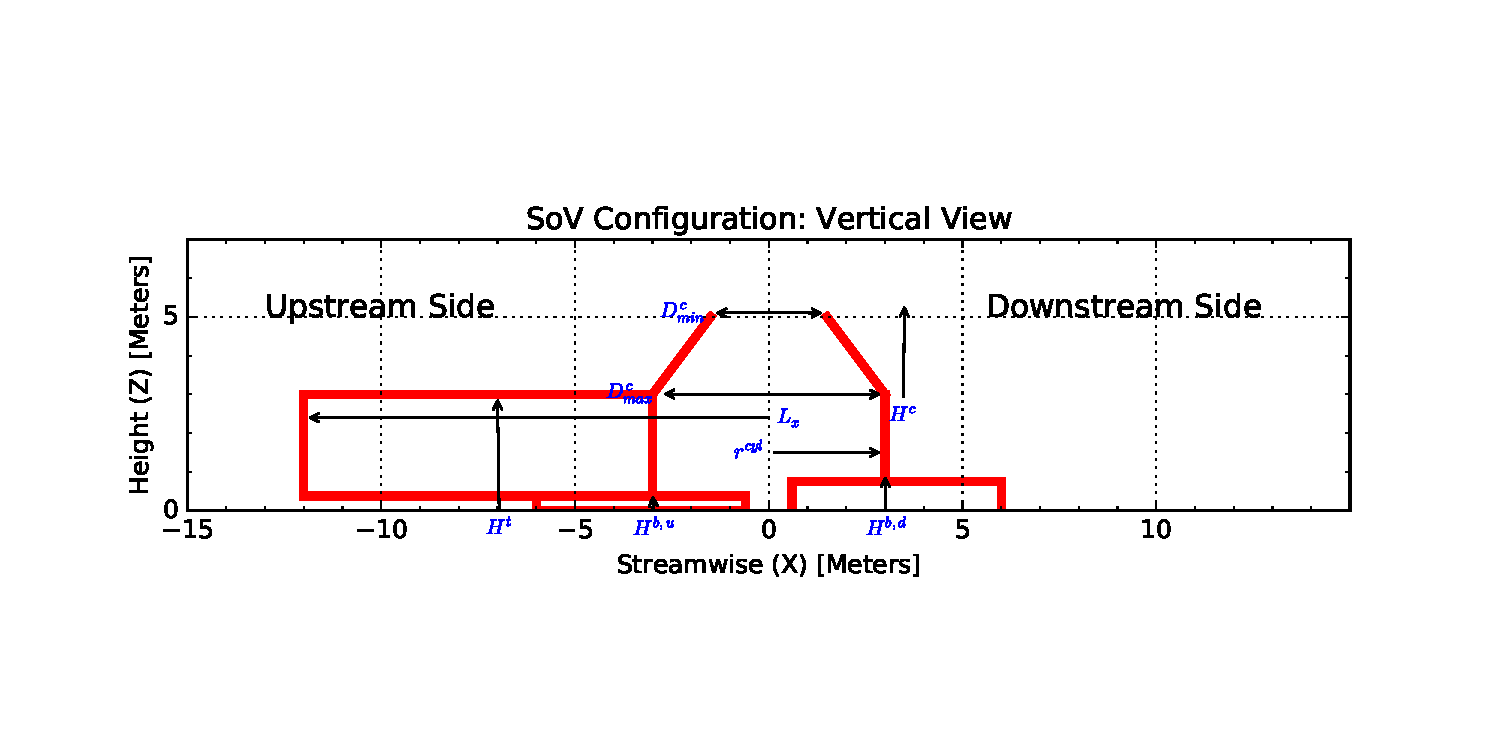
\includegraphics[width = 15 cm]{figs/vertical_design.pdf}
   \caption{A side view of the summer 2016 two tier vane design. The
     vanes are drawn in red. The difference in heights between lower
     tier vanes in front and back vanes is clearly visible. The turbine
     is placed at the top of the cone.}
   \label{fig:vertical_design}
  \end{center}
 \end{figure}

\begin{table}[]
 \caption{The values of the parameters shown in
 Figure~\ref{fig:vertical_design}, which is a side view of the SoV
 apparatus.} 
\centering
\begin{tabular}{l|l|l}
Name                        & Value [Meters] & Meaning                    \\
 \hline
$r^{\text{cyl}}$            &   3   & Radius of rigid cylinder \\
$L_x$                       &  12   & Furthest distance upstream of top	 tier vanes \\
 $H^t    $                  &   3   & Height of top tier vanes \\
 $H^{b,u}$                  & 0.375 & Height of bottom tier, upstream vanes \\
 $H^{b,d}$                  & 0.75  & Height of bottom tier, downstream vanes \\
 $H^{c}$                    &   2   & Cone Height \\
 $D^c_{\text{min}}    $     &   3   & Minimum cone diameter \\
 $D^c_{\text{max}}    $     &   6   & Diameter of cone at top of vanes\\
\end{tabular}
 \label{tab:side}
\end{table}

An optimal set of design parameters were determined and provided to the
experimental group, where they were instantiated as CAD designs by
Mr. John Culp at Georgia Tech. Images of the resulting model were generated
with FreeCAD~\cite{Falck} by the author and are
depicted in Figures~\ref{fig:top_down_cad} and \ref{fig:cad_skewed},
which show a top-down view and an angled 
view of the configuration. In both figures the bottom, top and cone are
clearly visible. This CAD design was used for
fabrication of the 2016 Field SoV Prototype. 

\begin{figure}[!htb]
  \begin{center}
   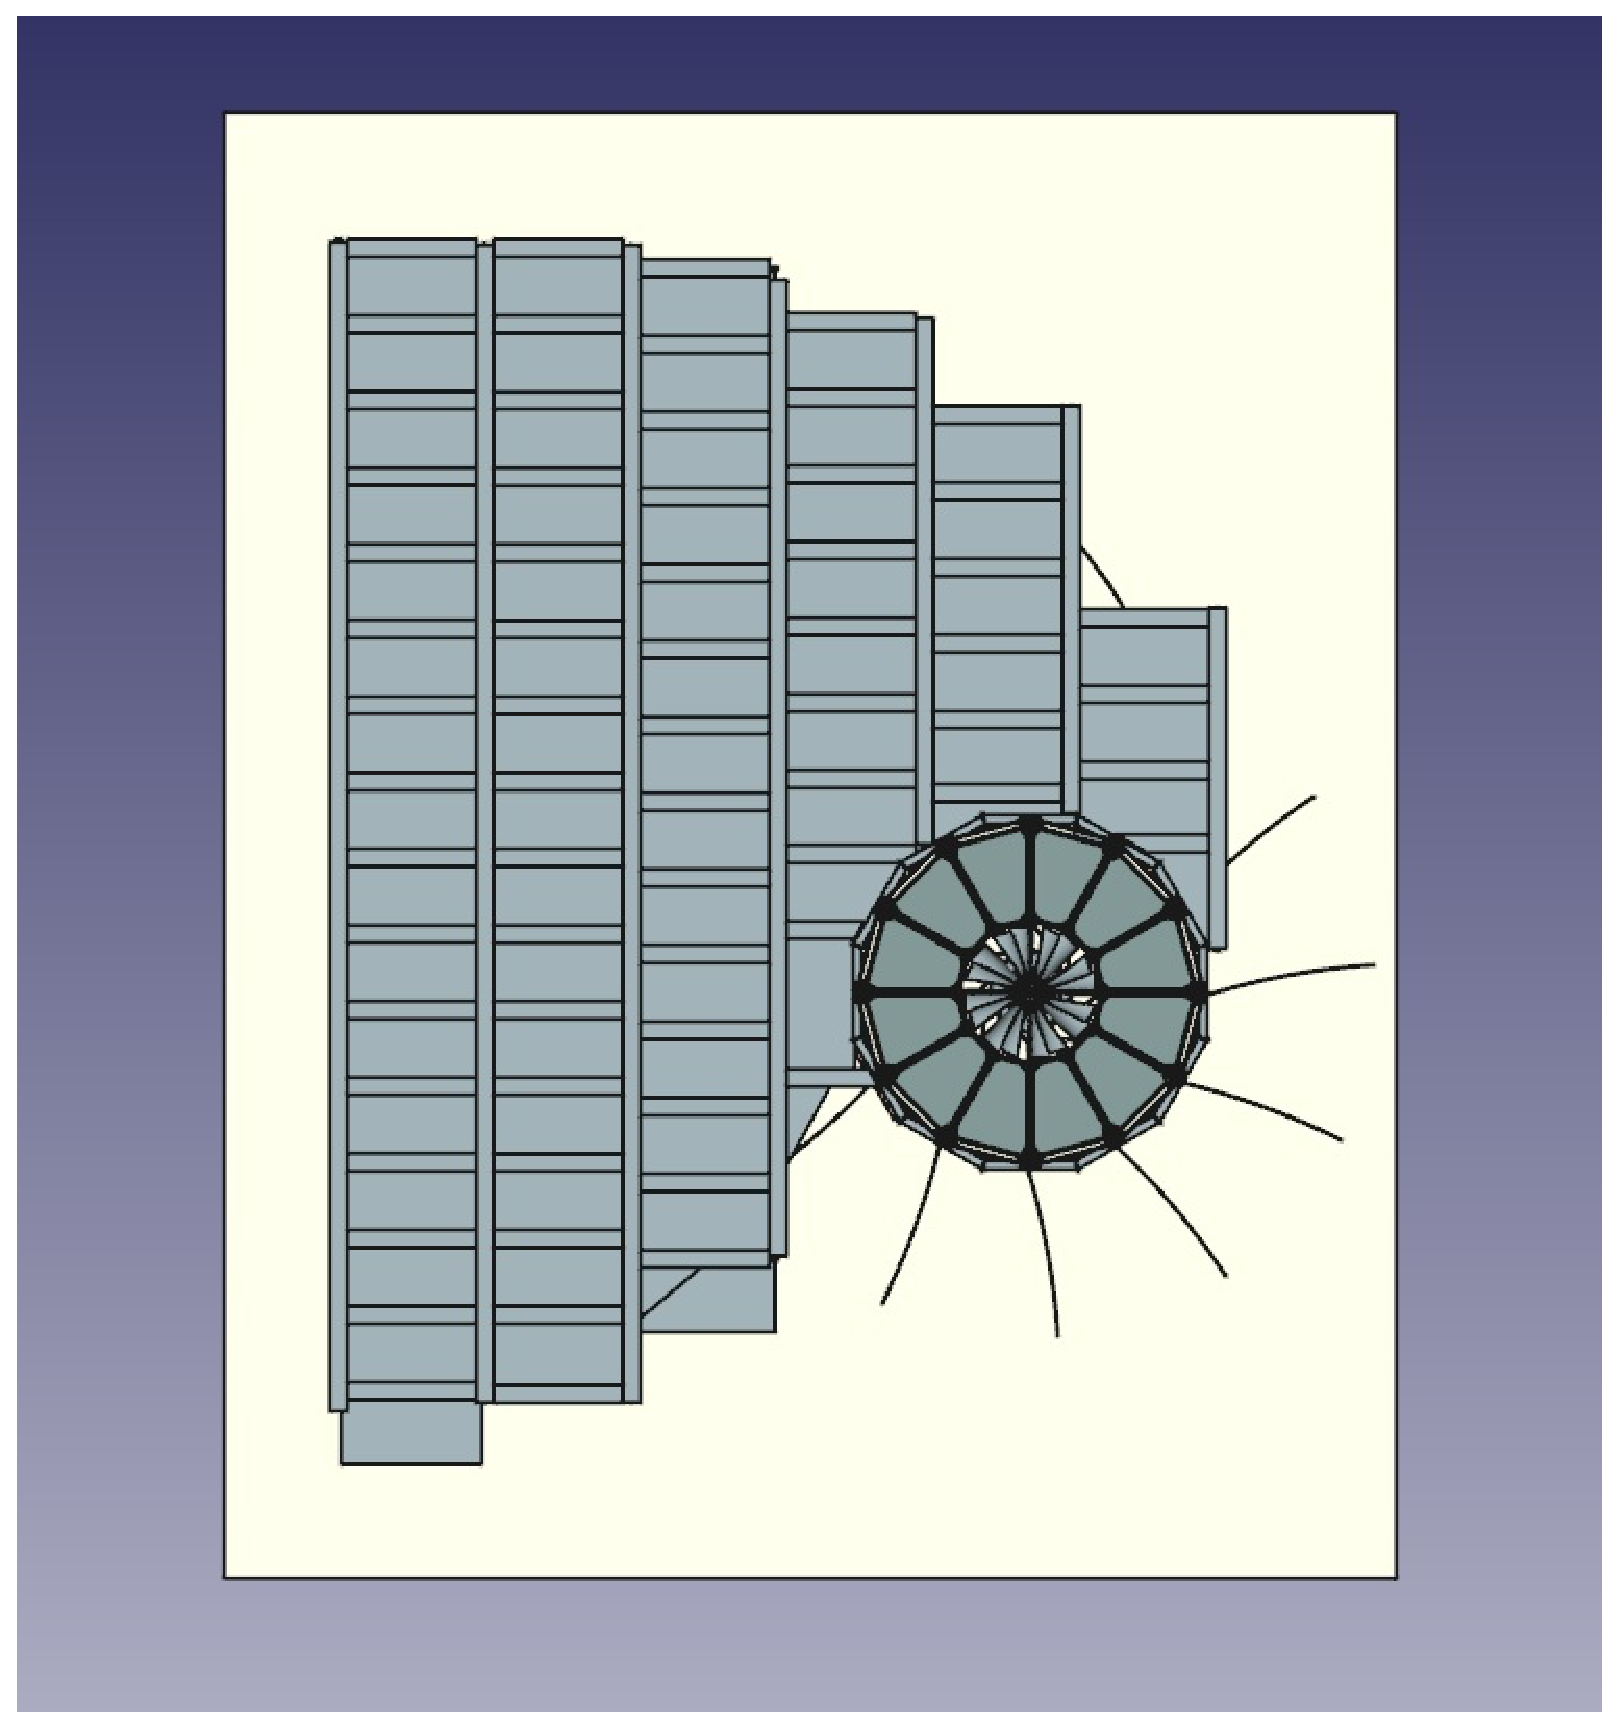
\includegraphics[width =0.7\textwidth]{figs/top_down_cad}
   \caption{A top view of the CAD drawing. The ``horizontal partitions''
   (designed to constrain the flow from leaving vertically) are clearly
   visible. In addition, the cone and turbine are also
   identifiable. Finally, the bottom tier vanes (which possess no
   horizontal partition) can be seen extending out the back of the
   device.} 
   \label{fig:top_down_cad}
  \end{center}
 \end{figure}

\begin{figure}[!htb]
  \begin{center}
   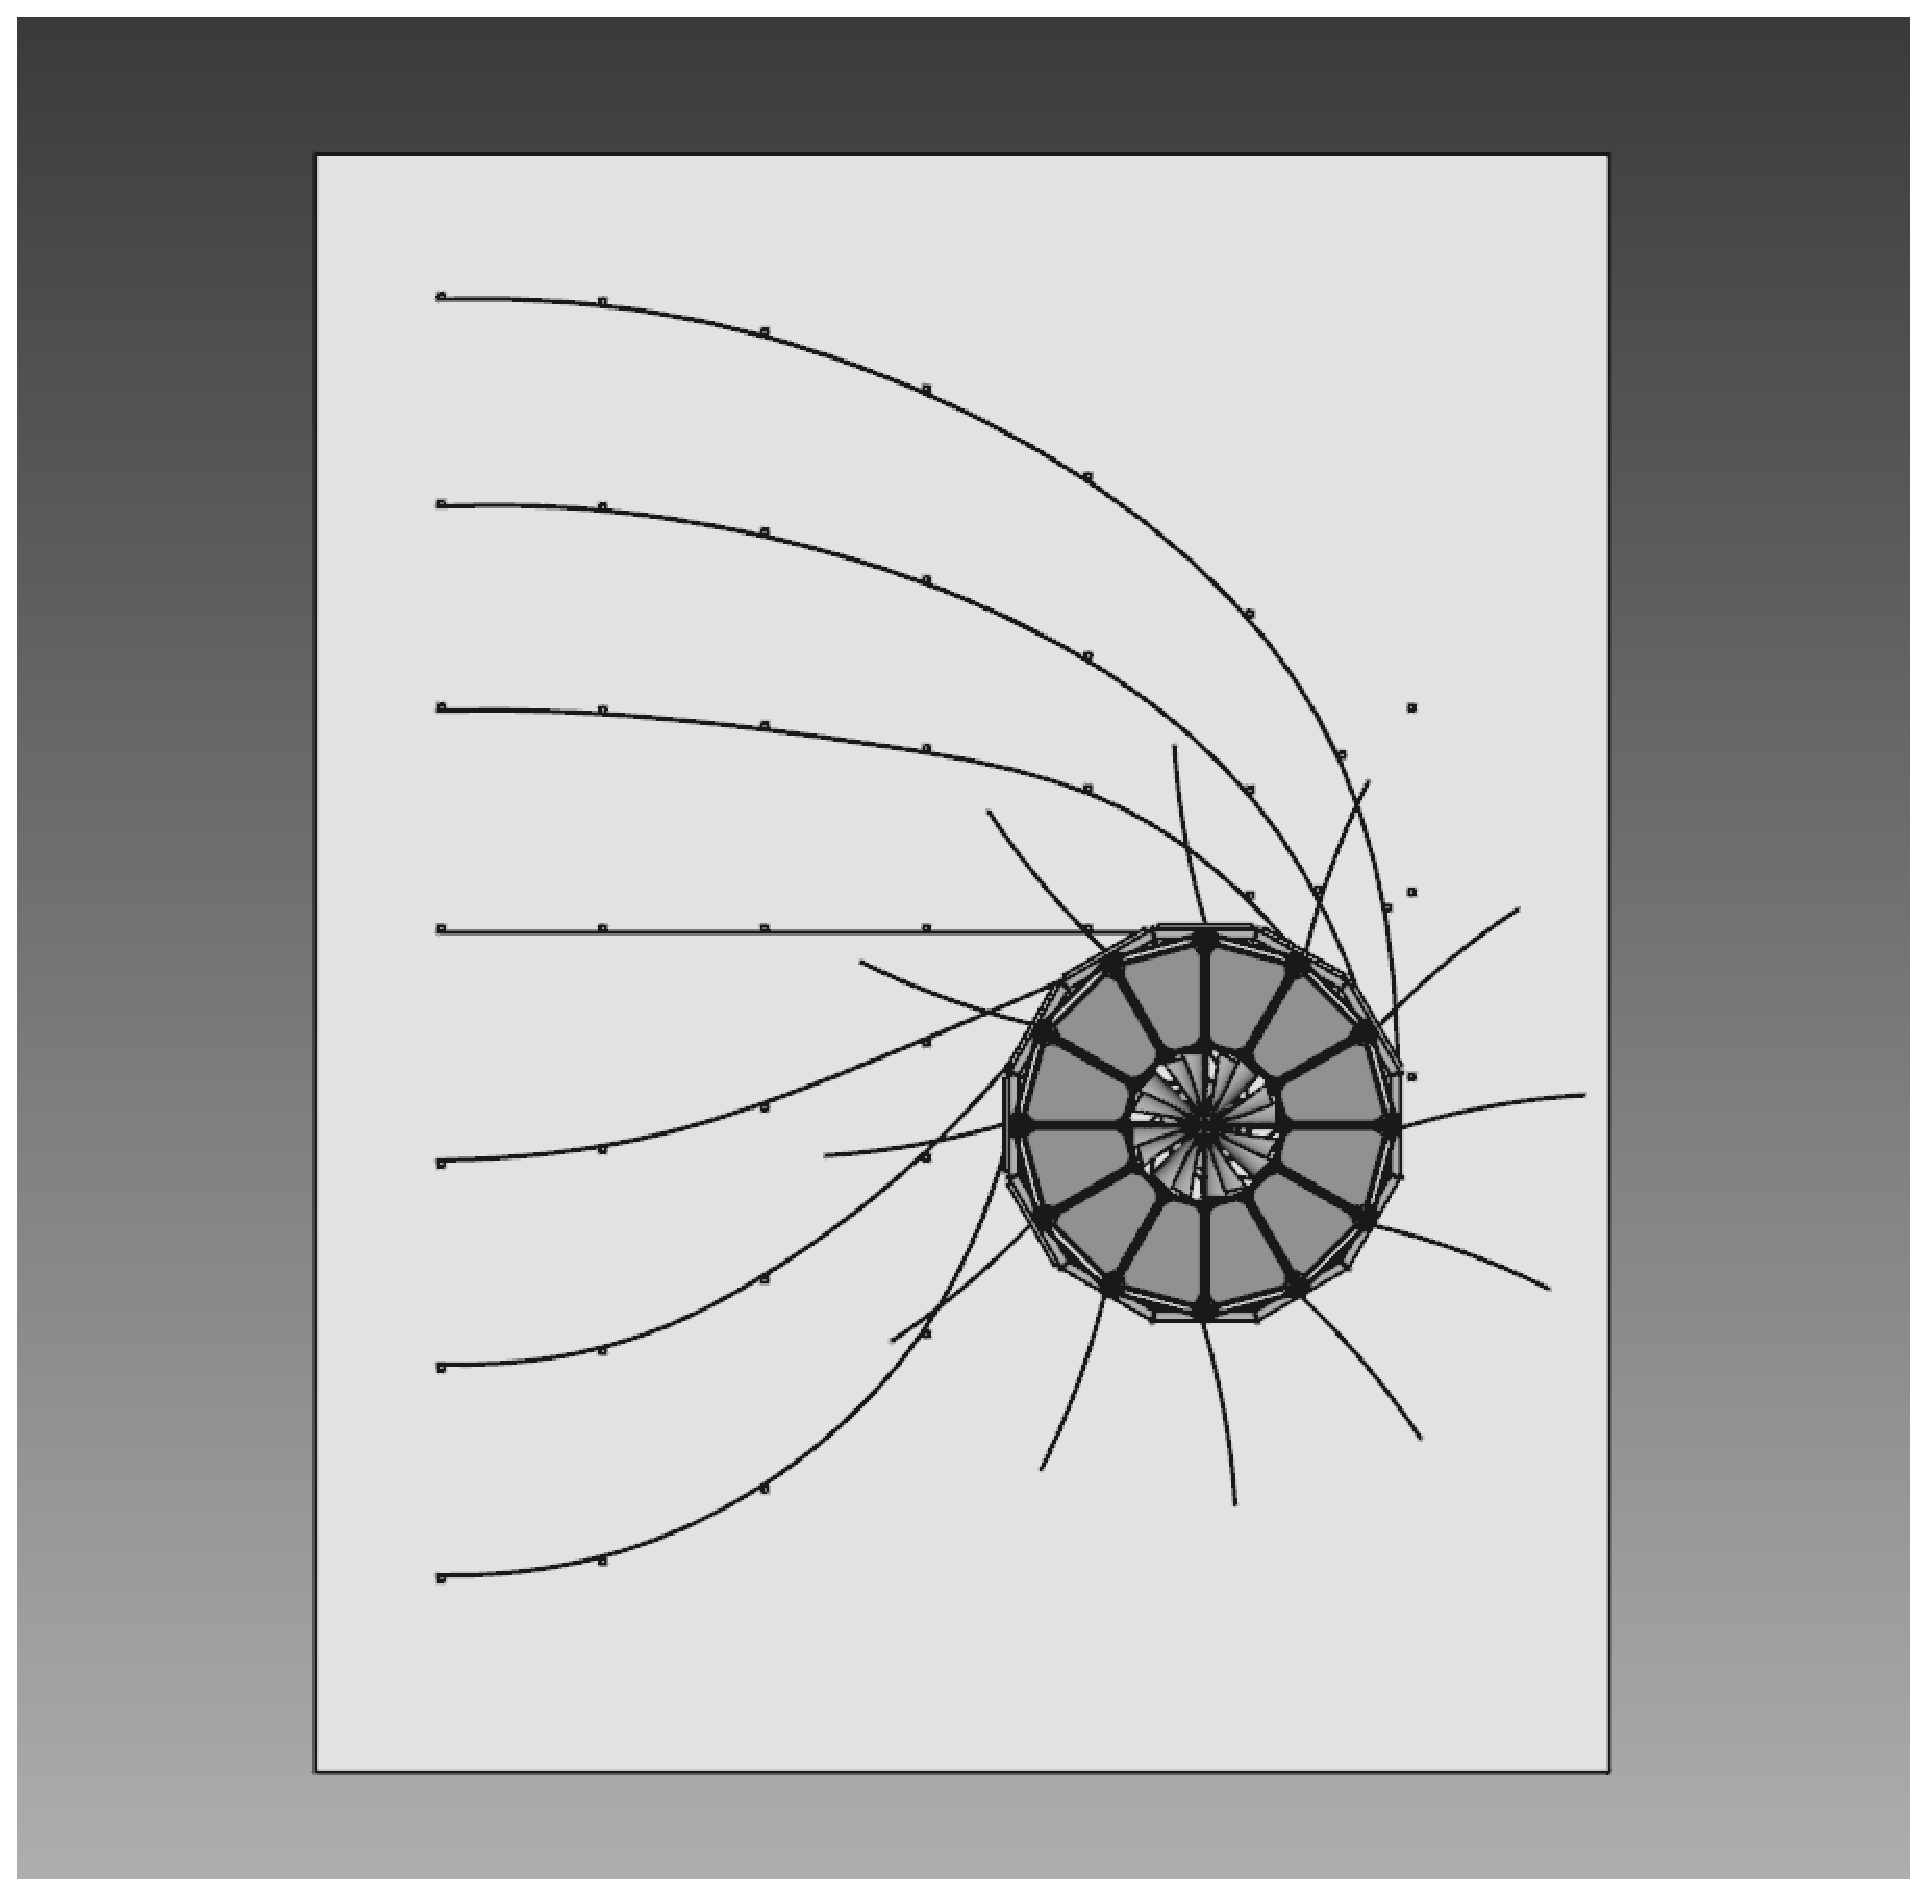
\includegraphics[width =0.7\textwidth]{figs/top_down_cad_notop}
   \caption{A top view of the CAD drawing, as in
   Figure~\ref{fig:top_down_cad}, but with the horizontal partitions
   removed. This provides a perspective on the second tier vanes, which
   extend out and in front (relative to the streamwise velocity) of the
   SoV.}
   \label{fig:top_down_cad_notop}
  \end{center}
 \end{figure}

\begin{figure}[!htb]
  \begin{center}
   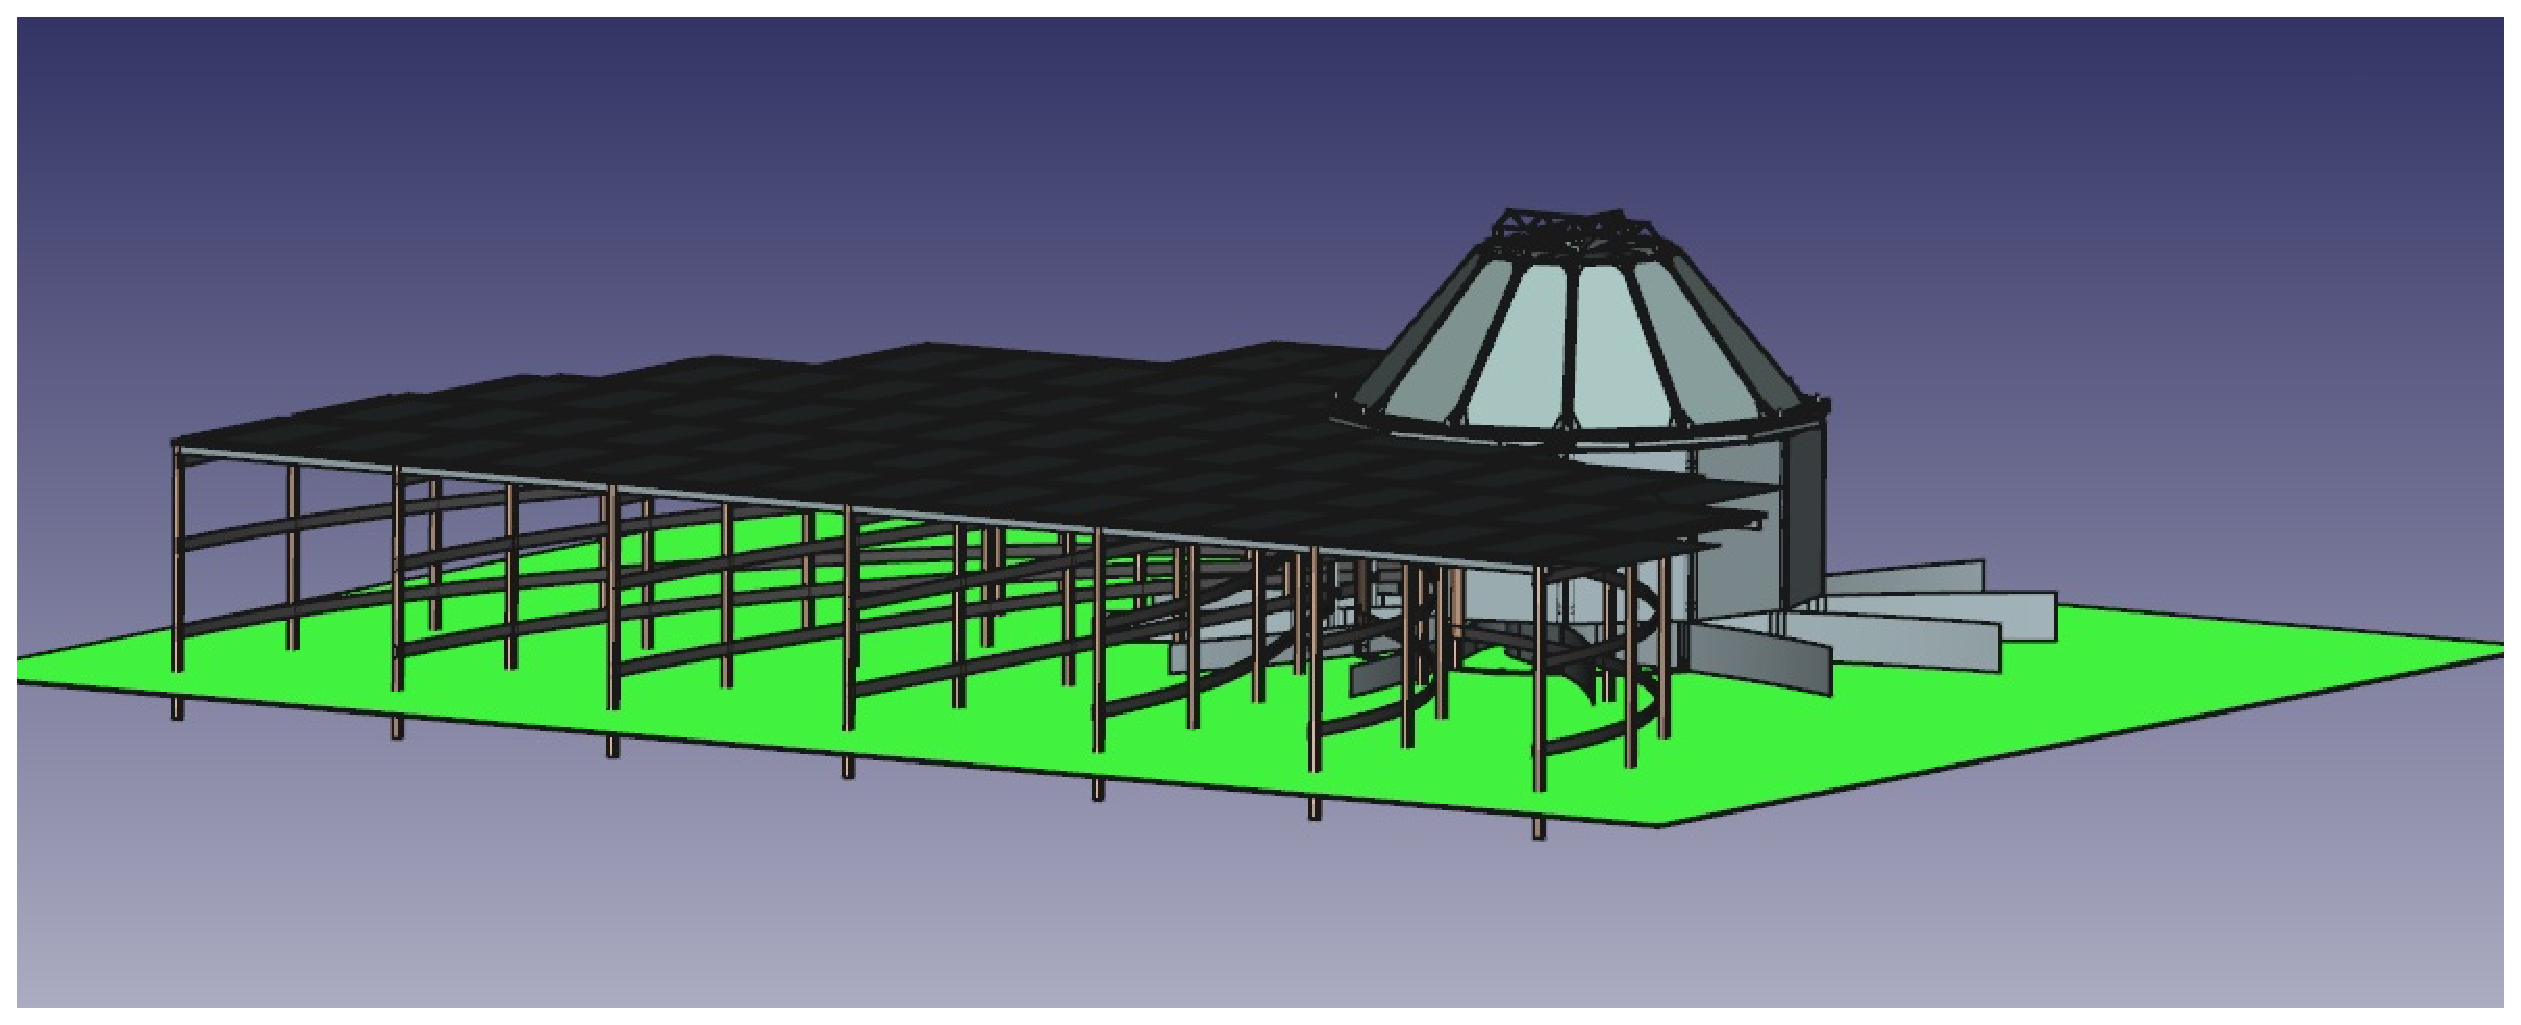
\includegraphics[width =0.7\textwidth]{figs/skewed_cad}
   \caption{A skewed view of the CAD drawings, which provides
   perspective on the height of the cone, the first and second tiers of 
   turning vanes, and the horizontal partitions.}
   \label{fig:cad_skewed}
  \end{center}
 \end{figure}

\subsection{Turning Vane Interpolation Functions}
\label{sec:interpolate}

The top tier design is now highly asymmetric, with a
large opening facing the incoming wind to capture incoming free stream
kinetic energy over a large area. The incoming flow enters the central
cylindrical area, where it spins and is driven out the top through the
cone. To enable these more asymmetric vane geometries for the top tier,
it was necessary to formulate a more general parameterization of the
vanes.

Previously, the vanes had a linear curvature function and were
axisymmetric. The new concept required the vanes to have an azimuthal
dependence so that they are aligned with the streamwise velocity upstream 
of the device, and then curve inward to spin the flow at the center of
the device. A linear vane curvature has
too few degrees of freedom to represent the design concept. 
Instead, vanes with elliptical shape are used. Each vane is a quarter of 
an ellipse or less. The minor axis of each ellipse is aligned in the inlet 
plane, and the vane terminates at the cylindrical boundary of the device interior 
at a nearly azimuthal angle. To implement this, the normal vector of the ellipse 
must be determined. 

This required use of implicit differentiation for the functional,

\begin{eqnarray}
 f(x,y)  =& \frac{(x-h)^2}{a^2} + \frac{(y-k)^2}{b^2} = 1, \\
 \nabla f(x,y) =& \frac{2 (x-h)}{a^2} + \frac{2 (y-k)}{b^2}\frac{dy}{dx} = 0, \\
 \frac{dy}{dx} =& -\frac{(x-h)}{(y-k)}\frac{b^2}{a^2}. 
\end{eqnarray}
Where h and k are the elliptic intercepts and a and b are the
eccentricity of the ellipse along each axis. The tangent vector along
the ellipse is then,  
\begin{eqnarray}
 %{\bf \hat t} = {\bf e_x} + \frac{dy}{dx}{\bf e_y}, \\
 {\bf t} =& {\bf e_x} + \frac{dy}{dx}{\bf e_y}, \\
 {\bf t} =& \underbrace{\frac{(y-k)}{b^2}}_{a_y} {\bf e_x} -
  \underbrace{\frac{(x-h)}{a^2}}_{a_x}{\bf e_y} \\
 {\bf t} =& {a_y} {\bf e_x} - {a_x}{\bf e_y}. 
\end{eqnarray}

Noting that the normal vector has the form, 
\begin{eqnarray}
 {\bf n} =& {a_x} {\bf e_x} + {a_y}{\bf e_y}, \label{eqn:a_x}\\
 {\bf n} =& \frac{(x-h)}{a^2} {\bf e_x} + \frac{(y-k)}{b^2} {\bf e_y}.
\end{eqnarray}

This now defines the normal vector. However, we need to determine the 
constants (namely, $k,b$) that define ellipses that capture the shape we
desire. We want to determine an ellipse that has a certain
slope, m, at a specific point,  $(x_0,y_o)$, which lies on the inner
radius (R) of the SoV apparatus. This is shown in
Figure~\ref{fig:elliptic_vane_concept}, and results in a system of four
equations,
\begin{eqnarray}
 \frac{(x-h)^2}{a^2} + \frac{(y-k)^2}{b^2} =& 1, \label{eq:ell1}\\
 \frac{(x_0-h)^2}{a^2} + \frac{(y_0-k)^2}{b^2} =& 1, \label{eq:ell2}  \\
 x_0^2 + y_0^2 =& R, \label{eq:ell3} \\
 -\frac{b^2}{a^2}\frac{(x_0-h)}{(y_0-k)} =& m. \label{eq:ell4} 
\end{eqnarray}
These equations express the fact that the ellipse intercepts two known
points, that the point $(x_0,y_o)$ lies on the inner radius of the
apparatus, and that the slope at this point is known. Assuming that
h, a, x, y, R and m are given, we have a system of four equations
(Equations \ref{eq:ell1}-\ref{eq:ell4}) with four unknowns,
$x_0,y_0,k,b$. This is, in principle, sufficient information to solve
this system. However, in practice, significant difficulties were
encountered. Inverting this system by hand is too complex and error
prone, and furthermore, Mathematica was unable to find a closed-form
solution. Numerous simplifications and additional constraints were added
to ensure that the system of equations were well-posed (a>b, for
instance), but the problem still resisted solution.\todo{rewrite}

 \begin{figure}[!htb]
  \begin{center}
   \includegraphics[width =0.95\textwidth]{figs/elliptic_vane_concept}
   \caption{The geometric problem for the elliptic vanes.}
   \label{fig:elliptic_vane_concept}
  \end{center}
 \end{figure}

The problem then, is that for a given location $(x,y)$ in space we are
unable to invert to determine the character of the ellipse that
intersects that point. Instead, we can pose the problem as discretizing
the arc along the inner radius of the vanes, we can generate data from
several curves that can be used to calibrate a 2D polynomial that will
smoothly vary in space. To accomplish this, we choose a series of
$x_0,y_0$ curves. For each unique ellipse defined by ($x_0,y_0,b,a,k$),
discretize at a uniform interval between $\left[-h,x_0\right]$, and
solve for the accompanying y-value, 
\begin{equation}
 y = -b \sqrt{1-\frac{(x-h)}{a^2}} + k. 
\end{equation}
One now has sufficient information to solve for the normal coefficients
$a_x$ and $a_y$ as defined in Equation~\ref{eqn:a_x}. This array of
coefficients specified at (x,y) are now fit to a 2D N\textsuperscript{th}
order polynomial. This has the form, 

\begin{equation}
 P(x,y) = \sum_{i=0}^N  \sum_{j=0}^N a_{i,j} x^i y^j
\end{equation}

where $a_{i,j}$ are coefficients of the polynomial which are selected by
minimizing the residual between the specified vane values and the
polynomial evaluated at that point. In other words, we find the
least-squares solution to a linear matrix equation, which is
under-determined. The solution to the equation $A {\bf x} = {\bf b}$ is
found by computing a vector ${\bf x}$ that minimizes the Euclidean
2-norm $|| {\bf b} - A {\bf x} ||^2$. The polynomials were computed in
separate python routines and 
resulted in a generated input file. This specifies the vane angle
function within the region of the vanes. This function is then used as
part of the input for the field runs (see Appendix~\ref{sec:archiving}
for more details on the input file environment). 
%
% http://docs.scipy.org/doc/numpy-1.10.0/reference/generated/numpy.linalg.lstsq.html
%

 % \begin{figure}[!htb]
 %  \begin{center}
 %   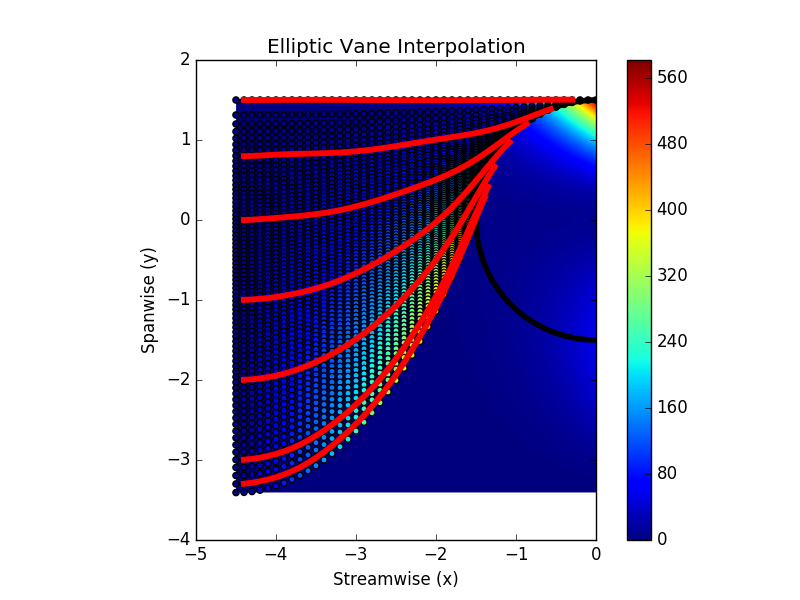
\includegraphics[width = 15 cm]{figs/bottom_interp}
 %   \caption{Top view of the interpolation function for the ``right
 %   side'' of the vanes on the top tier. The red lines are the data sets
 %   that provides the input data used to calibrate the two dimensional
 %   polynomial field. The black line is the inner radius of the SoV.}
 %   \label{fig:bottom_interp}
 %  \end{center}
 % \end{figure}

The polynomial order was selected to be 7\textsuperscript{th} because it
provided a good balance between accuracy and a desire to maintain as low
an order as possible. Furthermore, the vanes interpolation was split
into two components, for the ``left'' and ``right'' (from the perspective of a
person standing upwind of the SoV and looking at it) of the vanes in the
top tier. This was found to be the most effective way to ensure that the
polynomial remained accurate without requiring very high order
polynomials. The accuracy of the interpolated field was checked by
``drawing'' vanes by seeding a particle upstream of the field and then
manually integrating it through the field using the scipy integrate ode
packages and verifying visually that the vane had the correct
character. Figures~\ref{fig:top_design} and~\ref{fig:bottom_design} were
generated using this technique. 
% The ``right'' interpolated field is shown in
% Figure~\ref{fig:bottom_interp}.\todo{update python plots} 

%
% /h2/nick/src/code/python/poly_vanes
%

\section{Turbine Design}
\label{sec:turb_design}

In addition to the final vane design, a turbine design was developed and
tested over a range of design conditions. The design parameters defining
the turbine are listed in Table~\ref{tab:turbine}. The exploration of the
turbine design space was performed as outlined in
Figure~\ref{fig:opt_image}. The major design improvements are detailed
in Figure~\ref{fig:ut_turbine}. The ``initial guess'' was crude, with
flat plate drag polars and a poor 
initial guess for the blade angle of $\approx 10^{\circ}$. Later
designs use a higher blade angle often exceeding $40^{\circ}$. 
The design parameters that lead to the largest improvements in power
extracted were changes to the turbine blade geometry (from flat plate to
$180^{\circ}$ half cylinders to $90^{\circ}$ semicircles), optimization
of the blade angle and optimization of the turbine rotation rate. 
However, several other interesting improvements were also found, and are
detailed below.  

  \begin{figure}[!htb]
   \begin{center}
    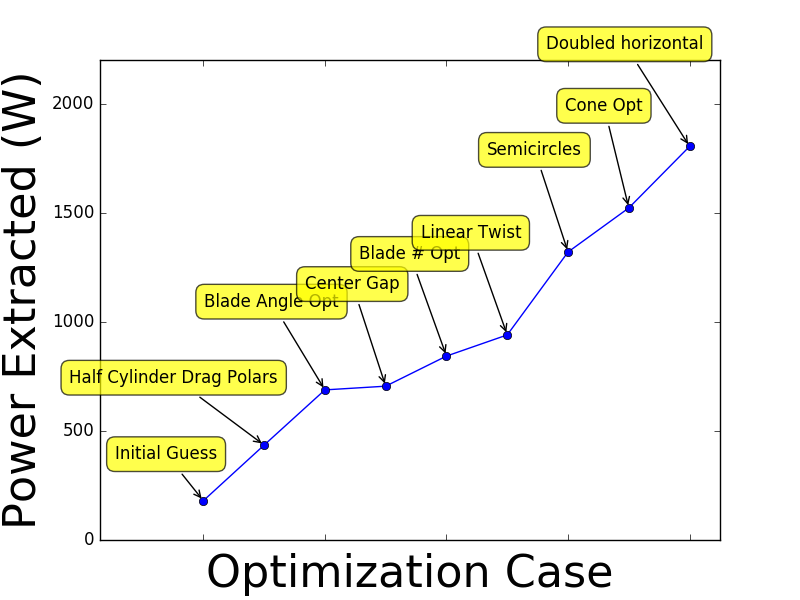
\includegraphics[width = 10 cm]{figs/turbine_opt}
    \caption{Initial turbine optimization before the coupling with the
    frozen flow. The ``initial guess'' was conducted with flat plate
    drag polars at a low blade angle ($\approx
    10^{\circ}$). Subsequent design improvements substantially improved  
    the power extracted, but this list constitutes only a ``greatest
    hits'' and the actual design improvements were highly iterative,
    with numerous runs of a particular parameter configuration yielding
    inferior power output. }
    \label{fig:ut_turbine}
   \end{center}
  \end{figure}

An open area in the center of the turbine was found to improve energy
extraction. In some cases, simulations showed a mild downward flow as
observed in the fully-developed thermal-only cases detailed in
Section~\ref{sec:thermal_only}. The present simulations do not form a
two-celled vortex, but an open center of the turbine is still
favorable. Similarly, while individual blades are not explicitly
represented in an actuator-disk model, the total projected area of
blades is a design parameter and can be optimized. This represents the
solidity or blockage, with more blades providing more surface area to extract
power from the fluid while simultaneously impeding the flow. A balance
between too much (a blocked off flow) and too little (too little blade
area to extract flow power) must be attained through optimization of the
controlling parameter, $B \, c$, the product of the number of blades and
each blade's chord length, as detailed in
Section~\ref{sec:actuator_disk}. 

Improvements to the turbine power extracted were also attained by adding
``twist''. In other words, the blade angle varies as a function of
radius, i.e. $\beta = \beta(r)$. The improvement in power extraction due
to a varying blade angle with radius is due to a changing distribution
of momentum flux. As both azimithal and axial velocities depend on the
circulation, $\Gamma$, so the optimal $\beta$ varies to capture
this. \todo{sufficient?} 

%Finally, cone improvement
After this initial exploration of the turbine design space, further
investigations were conducted in collaboration with Duane McCormick at
UTRC. This design was arrived at by comparisons between a ``frozen
flow'' optimization routine from UTRC  with the ``fully coupled'' CFD
described previously. This frozen 
flow Matlab code also used an actuator disk model as described in 
Section\ref{sec:actuator_disk}, and required the velocity profiles
immediately upstream of the actuator disk location from runs conducted
with and without the actuator disk present. Thus, the frozen flow
UTRC code was incapable of estimating the impact of a turbine on the
flow, and typically required updated velocity fields from the fully
coupled runs after several iterations. 
The UTRC code was not directly connected to the UT CFD code. Rather,
human intervention was required to prepare the velocity field outputs
from the UT CFD effort so that they could be used in the UTRC
code. Thus, the UTRC code would iterate through design parameters, and
then the CFD code was used as a higher fidelity confirmation. The UTRC
frozen flow optimization was largely consistent with the fully coupled
CFD prediction (see  Figure~\ref{fig:UTRC_turbine}, below). This has
resulted in two final rotor designs, with and without twist. This was
because the experimental team was not certain that a twisted design
would be feasible. Regardless, the twisted rotor was always predicted to 
out-perform the zero-twist rotor.  
The peak power extracted is predicted to be 2.14 kW for the rotor
with twist, and slightly more than 1.51 kW for a rotor with no twist. 
% The load on the turbine
% is predicted to be modest, at 20 ft-lbs. 
This indicates that the twisted rotor design is extracting 44\% of the
available power from the flow. This is an efficiency: the power
extracted by the turbine ($P_{\text{Turbine}}$) from the kinetic energy
flux ($\dot{\text{KE}}$) through the device, e.g.
\begin{equation}
\eta_{\dot{\text{KE}}} = \frac{P_{\text{Turbine}}}{\dot{\text{KE}}}. 
\end{equation}
The Betz-limit, which of limited use due to its
neglect of rotation, places an upper bound of 59.3\% of the
power contained in the flow that might be extracted. Then we can
consider a ``Betz-efficiency'', which is the ratio of the available
kinetic energy flux extracted versus this bound, 
\begin{equation}
 \eta_\text{Betz} = \frac{\eta_{\dot{\text{KE}}}}{59.3 \%}
\end{equation}
This indicates a Betz-efficiency of $\approx 75\%$, which is roughly
consistent with the measured efficiency of modern wind turbines. 
All of these results are for the $90^{\circ}$ circular-arc
blade, as shown in Figure~\ref{fig:90_drag}. 
% after duane

  \begin{figure}[!htb]
   \begin{center}
    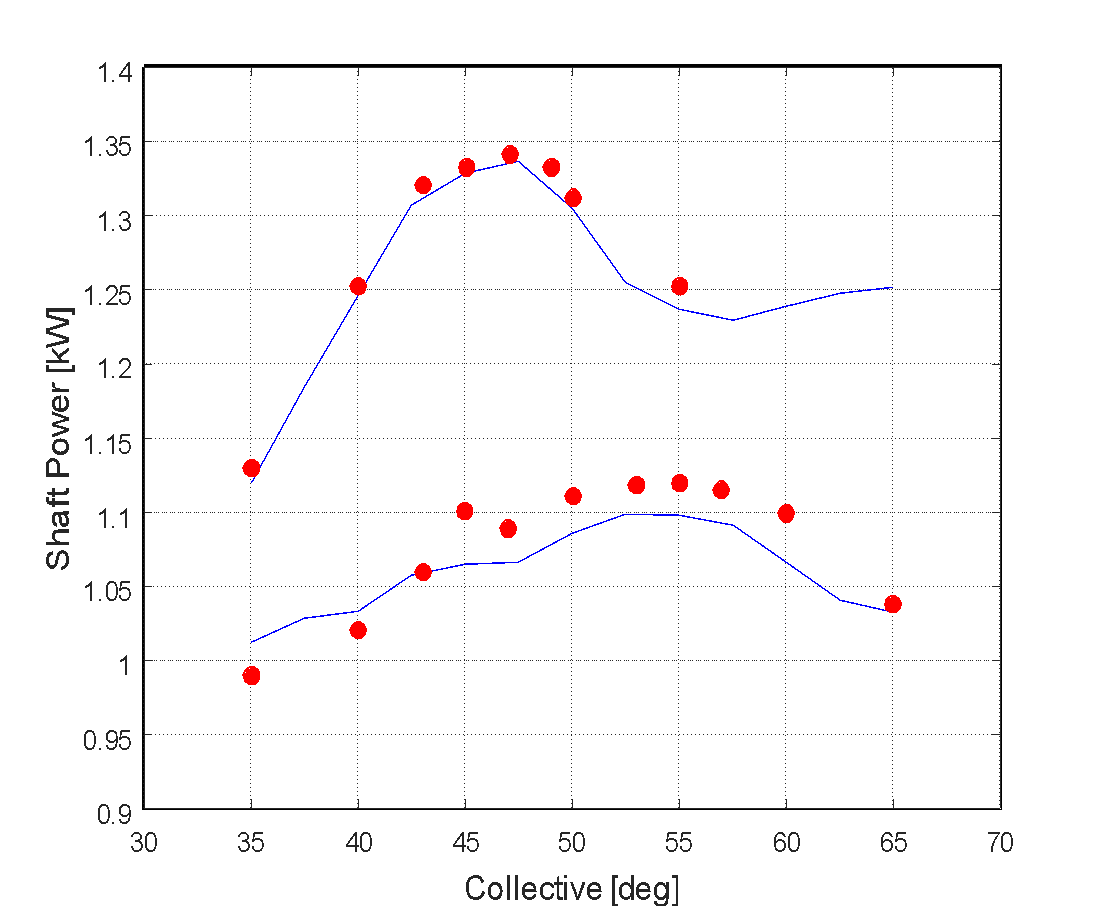
\includegraphics[width=.8\linewidth]{figs/utrc_plot}
    \caption{The power extracted by the rotor predicted by the CFD
    (dashed line) and frozen flow (solid line) for a range of rotor
    collective angles. The higher lines (red circles) are for blades
    with twist, and the lower (blue diamonds) are for constant blade
    angle runs, which was always  inferior in terms of power
    extracted. In general the frozen flow closely tracks the CFD.}
    \label{fig:UTRC_turbine}
   \end{center}
  \end{figure}

The proposed turbine design is shown in Table~\ref{tab:turbine}. Note
that the design parameter $Bc $ is actually the number of blades
multiplied by the chord length. As detailed in
Section~\ref{sec:actuator_disk}, this is the actual parameter of
interest in the actuator disk formulation. For fabrication, this was 
decided to correspond to eight blades with a chord length of 0.45 meters
each. %\todo{discuss twist}  

\begin{table}[]
\centering
 \caption{The parameters for the optimized turbine design.}
\begin{tabular}{l|l|l|l}
Name                & Current Value    & Symbol           & Comments \\
 \hline
Outer Blade Angle & $70^{\circ}$ & $\beta_{\text{outer}}$  & linear twist between \\
Inner Blade Angle & $47^{\circ}$ & $\beta_\text{inner}$    & 
	     $\beta_\text{inner},\beta_\text{outer}$ \\ 
\# blades * Chord Length & 3.6 meters  & $Bc $ &  \\
Turbine rotation rate & 4.0 rad/sec  & $\omega$         &  \\
Blade Outer Radius  & 1.5 meters   & $B_\text{outer}$ &  \\
Blade Inner Radius  & 0.3 meters   & $B_\text{inner}$ &  \\
Height of turbine   & 4.5 meters   & $H_B$            & Height of turbine \\
\hline
\end{tabular}
 \label{tab:turbine}
\end{table}

As mentioned previously, the frozen flow and fully coupled CFD
agree. However this is only for rotor loadings close to those in the
coupled CFD. Substantial errors tended to appear in the frozen flow
predictions with parameters far from the coupled CFD. In some cases, the
limitations of the frozen flow optimization were significant. For
instance, the frozen flow model would consistently predict larger power
output at higher RPM. However, several attempts to extract more power at
larger RPMs would cause a breakdown of SoV flow in the coupled CFD
model, which resulted in the flow power dropping by more than an order
of magnitude.%\todo{add turbine flow pictures} 

  \begin{figure}
   \centering
   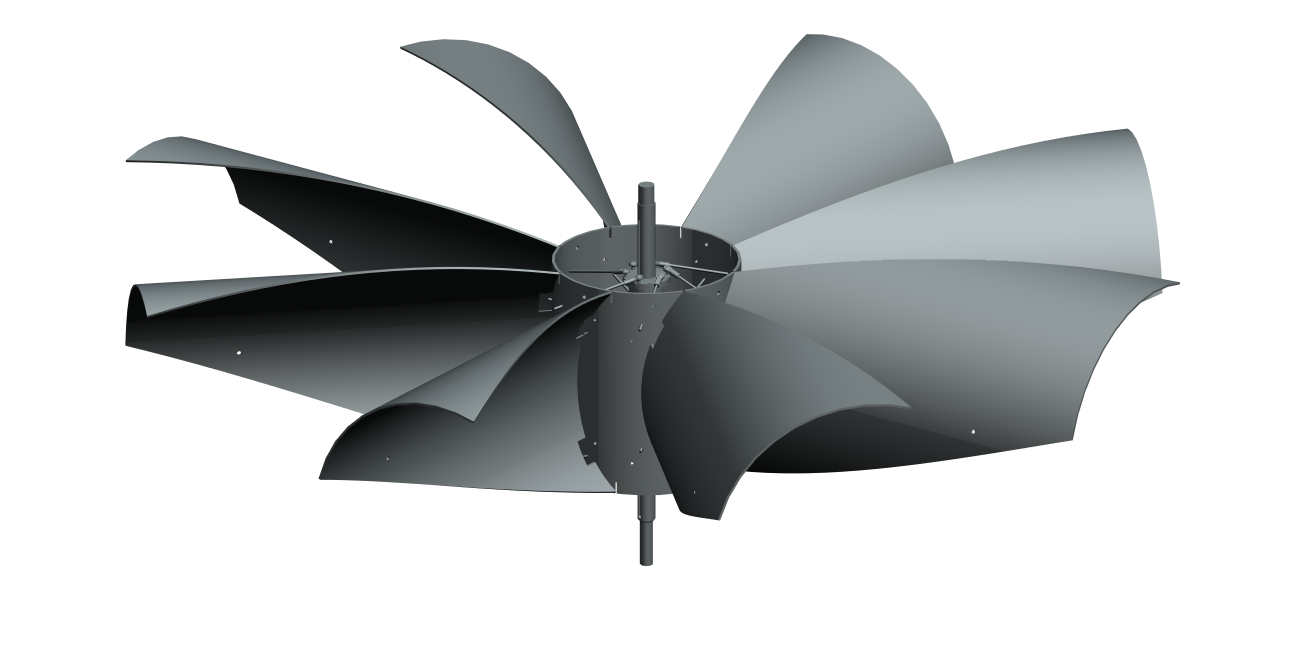
\includegraphics[width =0.45\textwidth]{figs/rotor_assem_oblique_1}
   \hfill
   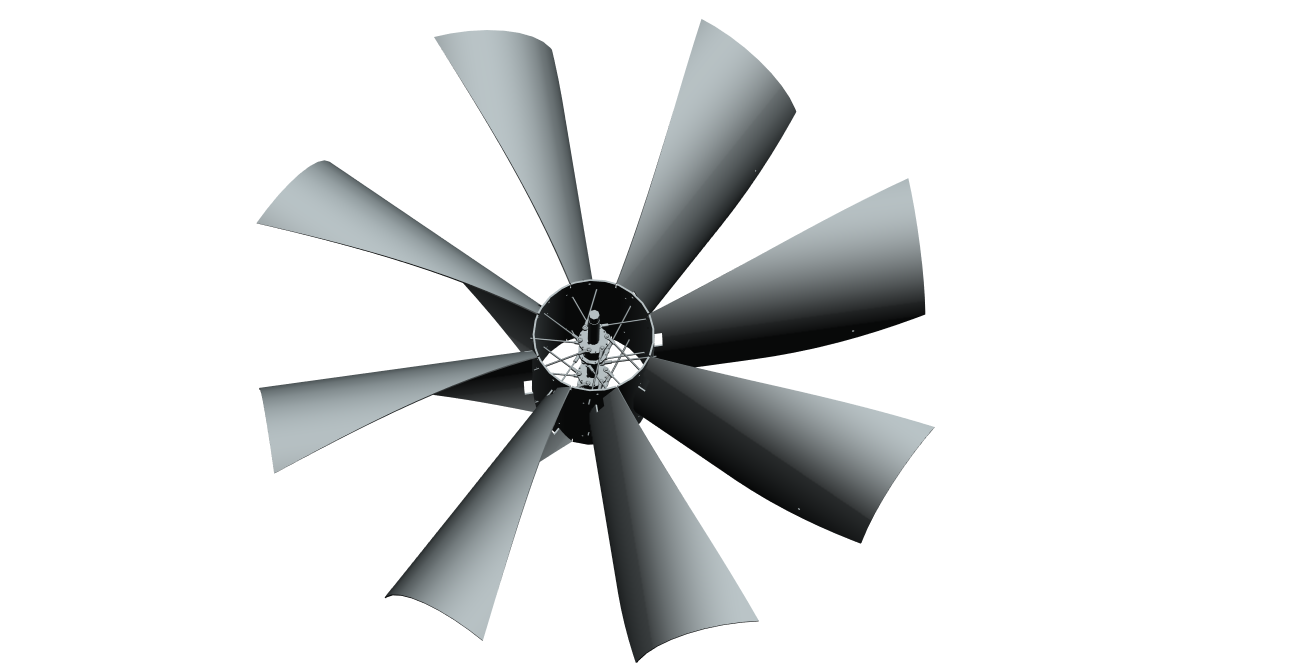
\includegraphics[width =0.45\textwidth]{figs/rotor_assem_oblique_2}
   \\
   \vspace{1em}
   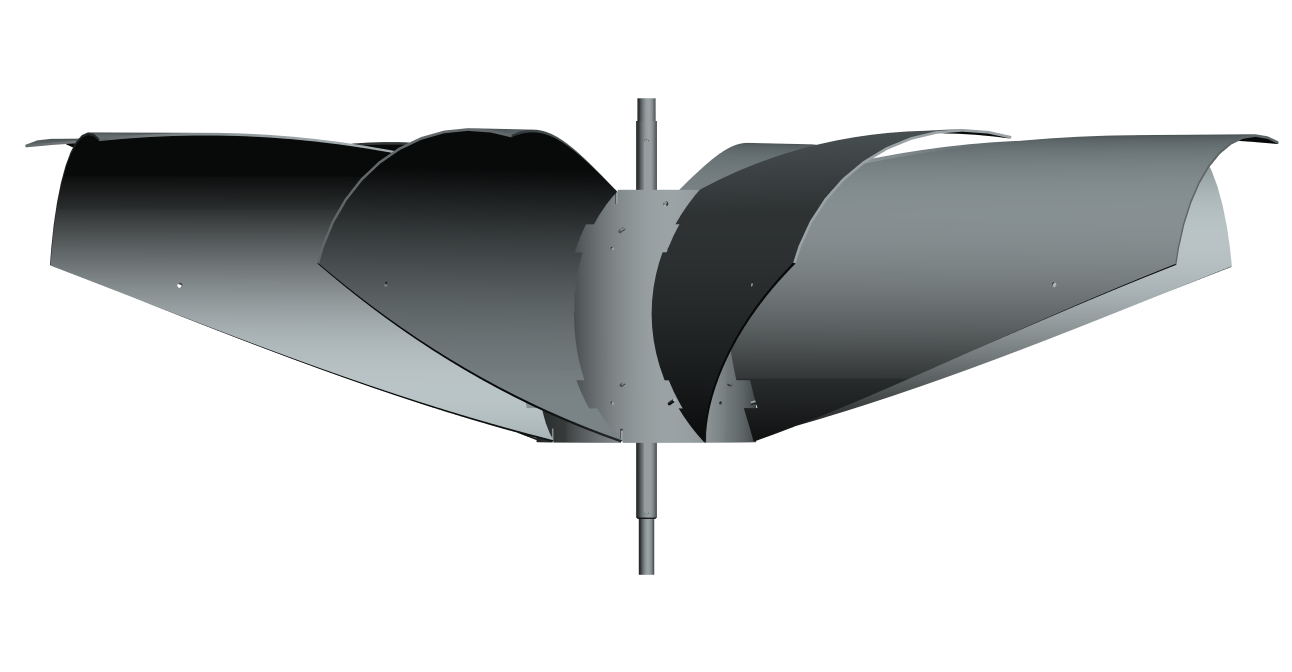
\includegraphics[width =0.45\textwidth]{figs/rotor_assem_side_render}
   \hfill
   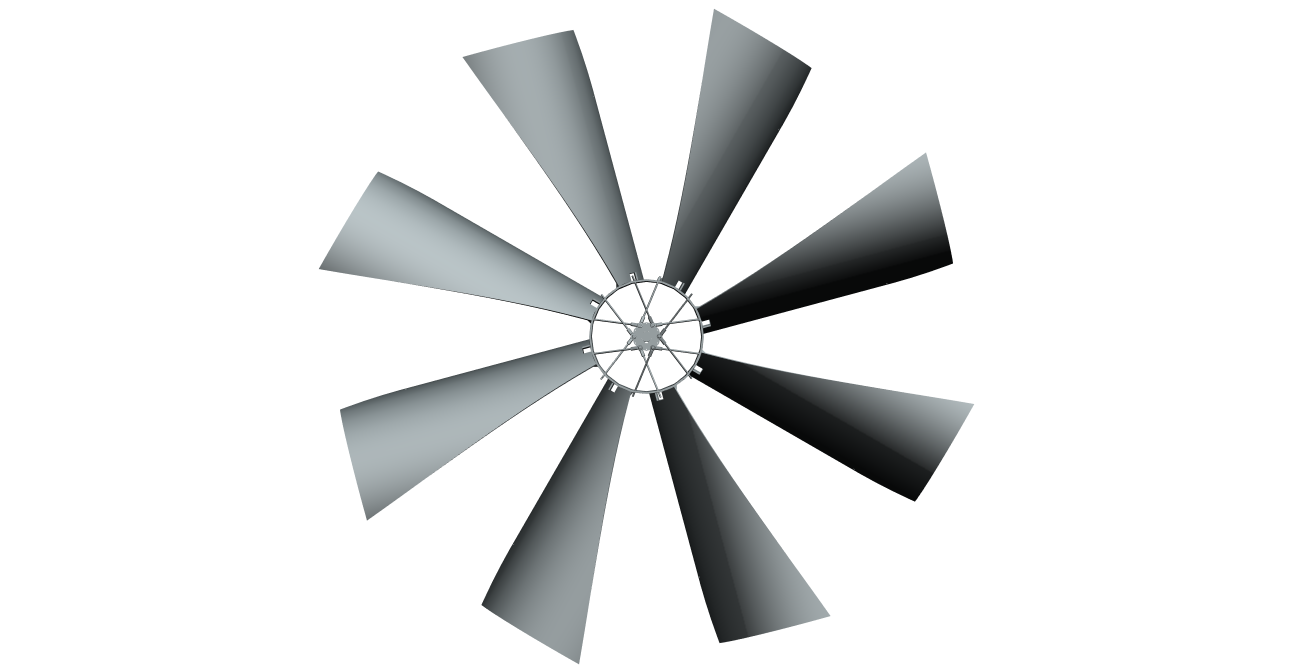
\includegraphics[width =0.45\textwidth]{figs/rotor_assem_top}
   \\   
   \caption{CAD design images of the turbine. The CAD designs were
   created by the team at Georgia Tech based on the design
   specifications from the CFD performed by the author. The images were
   created from these CAD files by the author using
   FreeCAD\cite{Falck}.}  
   \label{fig:cad_turbine}
  \end{figure}


  \begin{figure}
   \centering
   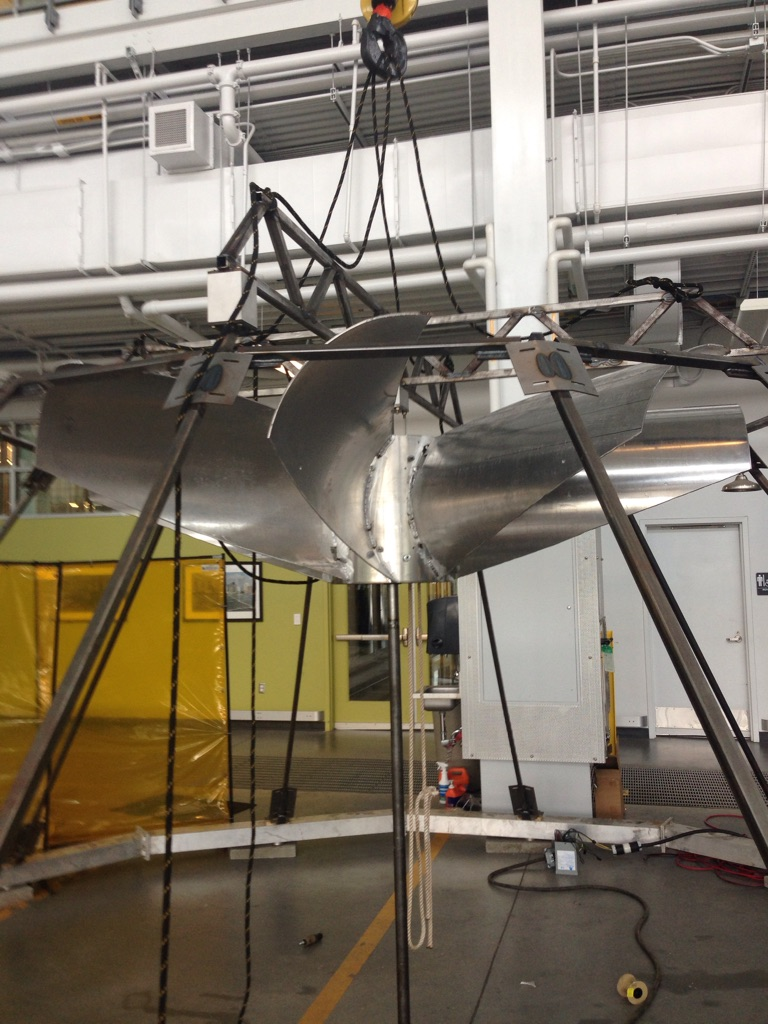
\includegraphics[width =0.45\textwidth]{figs/turbine_built}
   \caption{The fabricated turbine. The cone superstructure is also
   visible.} 
   \label{fig:turbine_built}
  \end{figure}

%Shortcomings -- \todo{finish me}
%Designed for axisymmetric flow. 
%No wake correction as depicted in Section~\ref{subsec:wake_loss_model}.    

\section{Scenario Parameters}
\label{subsec:scenario_param}

With the system geometry defined, we need only impose the boundary
conditions defined in Section~\label{sec:bc} to have defined our
scenario of interest. However, as with the validation case shown in
Section~\ref{sec:field_val}, significant uncertainty exists in the
scenario parameters that define the ambient thermal and wind
conditions. Some discussion of the scenario parameters is therefore
warranted. 

The thermal boundary layer was set based on data gathered by 
the Georgia Tech team in Arizona on June 9th, 2014. The raw data
presented in Figure~\ref{fig:thermal_profile_fit} is the average from
four vertical temperature profiles take at different times during a
single day. The measurements were gathered between 9:49 am and 1:43
pm\cite{ann_comm}.  

A particular challenge is that the closest measurement was taken by a 
thermocouple 1 mm above the pavement. Thus, the surface temperature was
not directly measured. To estimate 
$T_0$ and $\Delta T$, the thermal profile was fit with a least squares
minimization of the residual between Equation~\ref{eq:bl_t} and the
experimental data. The resulting profile is plotted in
Figure~\ref{fig:thermal_profile_fit}. The sparsity of experimental data
near the surface is quite clear from this profile. The fitted profile is
then evaluated at $x=0$ to determine the ground temperature. Based on
this calculation, a temperature difference of 30 Kelvin was determined.   

 \begin{figure}[!htb]
  \begin{center}
   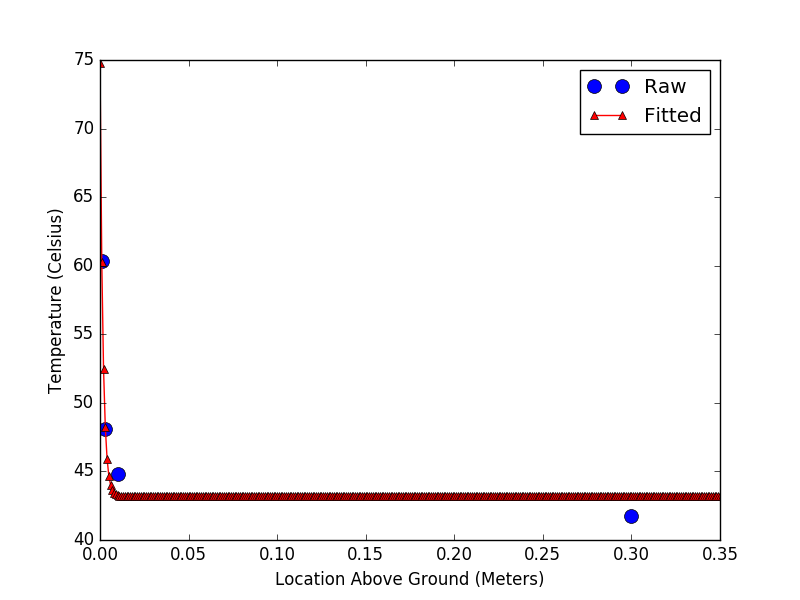
\includegraphics[width = 15 cm]{figs/fit_zoomed}
   \caption{The raw thermal boundary layer data (blue circles) plotted
   against the fitted boundary layer profile (red triangles). The
   paucity of experimental data undermines the fit's accuracy to
   anything more than a plausible location for the actual wall
   temperature. }  
   \label{fig:thermal_profile_fit}
  \end{center}
 \end{figure}

In addition to the thermal profile, the incoming wind velocity was
needed. Thankfully, wind measurements were also performed by the
experimental team in the field during the June, 2014 test. A one hour
time series was captured for both day and night as measured by the sonic
anemometers. These data are plotted in
Figure~\ref{fig:wind_speed_estimate}. The wind speed was sampled at a 
rate of 0.5 Hz, and the traces are plotted for one hour (for
both the day and night). 

 \begin{figure}[!htb]
  \begin{center}
   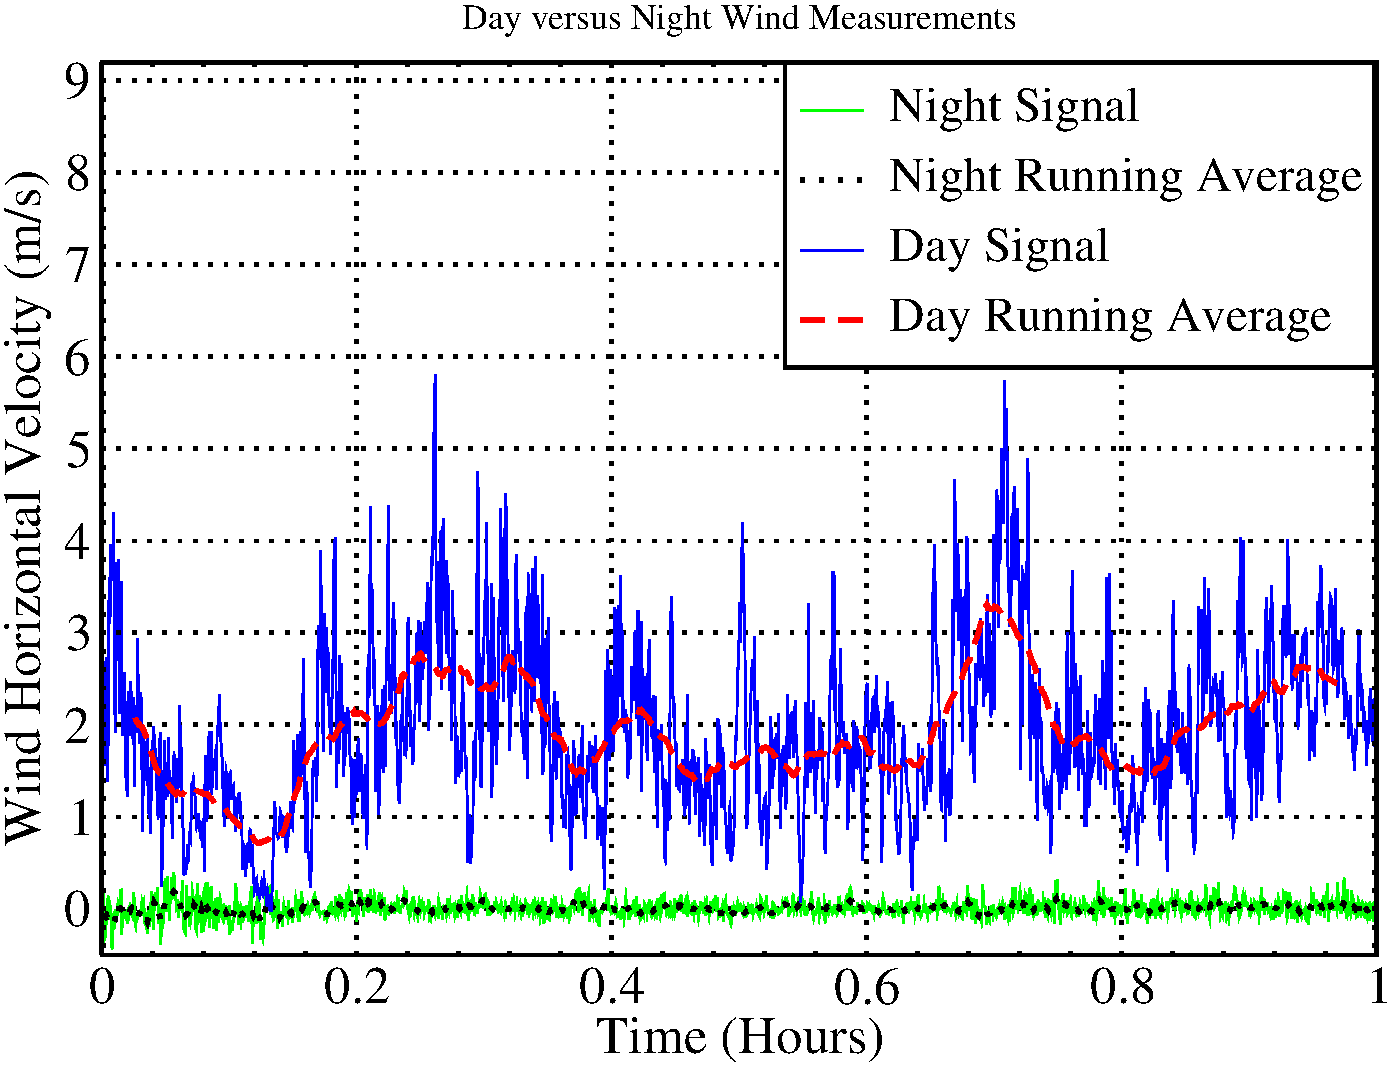
\includegraphics[width=.7\linewidth]{figs/wind_measurements}
   \caption{Wind Speed Measurements from the June 2014 field test.}
   \label{fig:wind_speed_estimate}
  \end{center}
 \end{figure}

Several observations can be made from this data. There is essentially no
mean flow at night, but during the day the winds are significant,
with a mean velocity of about two meters per second and fluctuation that
reached nearly six meters per second. 
%The wind profile at both day and
%night possessed rapid, small scale fluctuations in time which were not modeled. 
%Also note that the daytime
%wind always  has non-zero mean, and the average horizontal velocity during the day is
%between 2-3 m/sec.  

The wind direction was also monitored, and showed little variation. 
This is shown in Figure~\ref{fig:wind_direction}. It was therefore
assumed that the wind had a constant heading and constant speed during
the simulations. Furthermore, discussions with the field team indicated
that wind heading over several years of field tests were relatively
consistent. This was part of the motivation for the introduction of an
asymmetric vane configuration, since if the wind direction changed daily
(for instance) it would render an asymmetric design useless, unless it
could easily be realigned with the free stream velocity. 

 \begin{figure}[!htb]
  \begin{center}
   \includegraphics[width=.7\linewidth]{figs/wind_direction}
   \caption{Wind direction measurements from the June 2014 field test.}
   \label{fig:wind_direction}
  \end{center}
 \end{figure}


% monin obuhkov should deal with this, no?
%It may well be that even in the "thermal only" cases there could be
%significant, zero mean turbulence (perhaps like grid turbulence)
%contributing from the ambient surroundings. 

\section{Solution Structure of the Field Configuration}
\label{subsec:field_predict}

\begin{figure}[!htb]
  \centering
  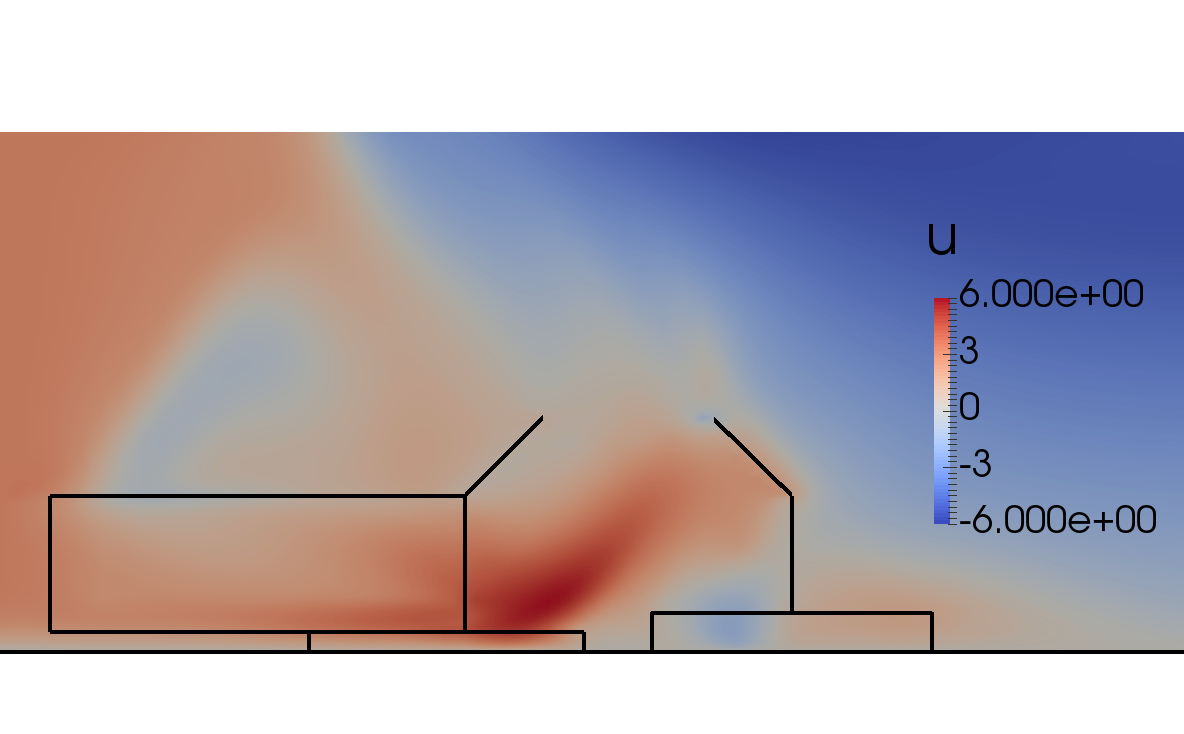
\includegraphics[width=.47\linewidth]{figs/u_field_vert}
  \hfill
  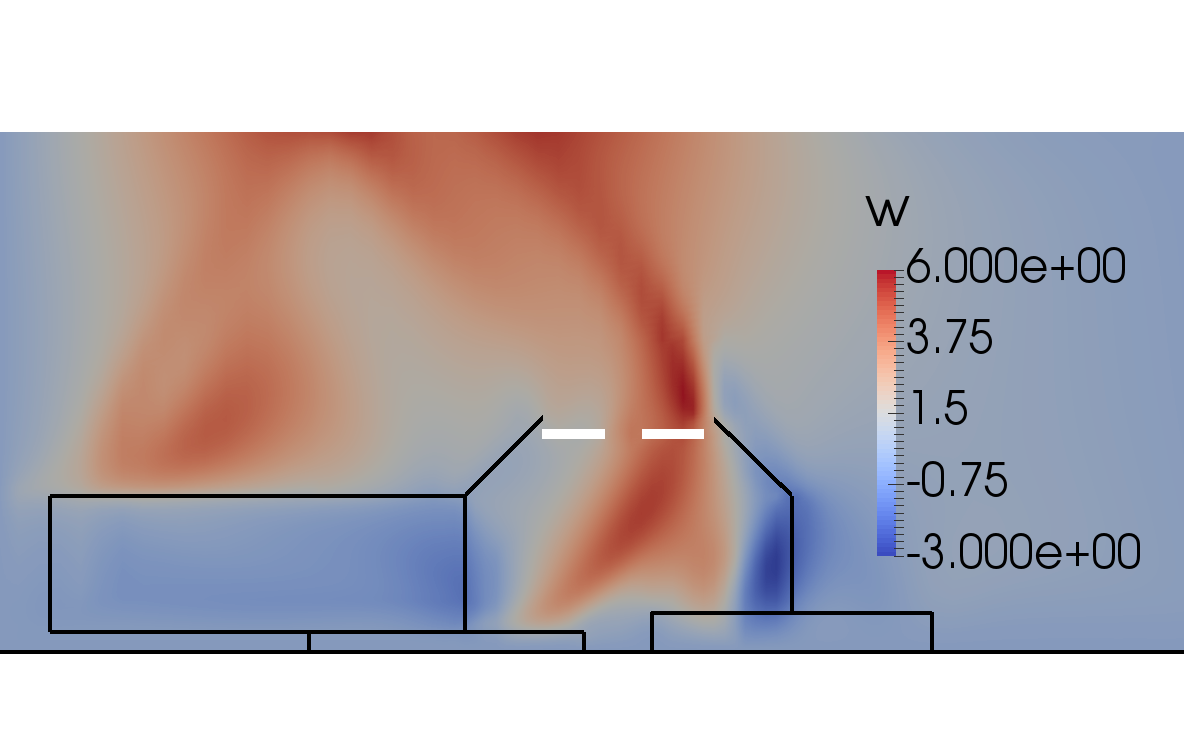
\includegraphics[width=.47\linewidth]{figs/w_field_vert}
  \\
  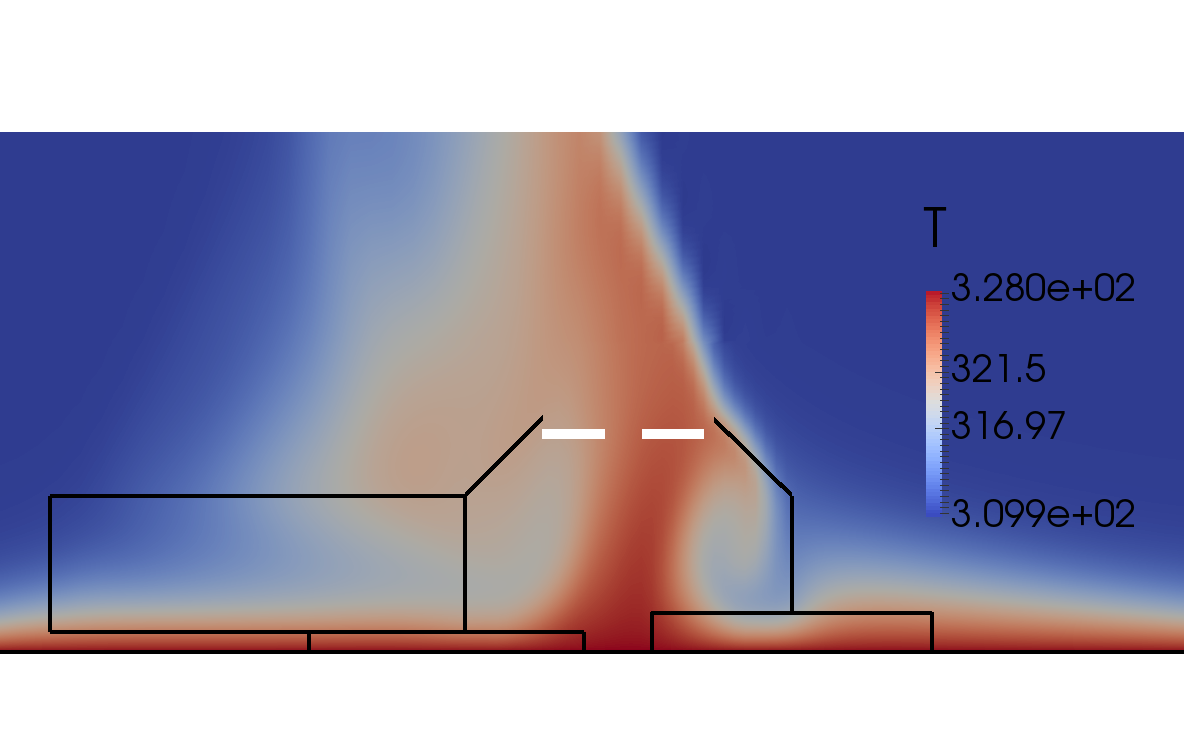
\includegraphics[width=.47\linewidth]{figs/T_field_vert}
  \hfill
  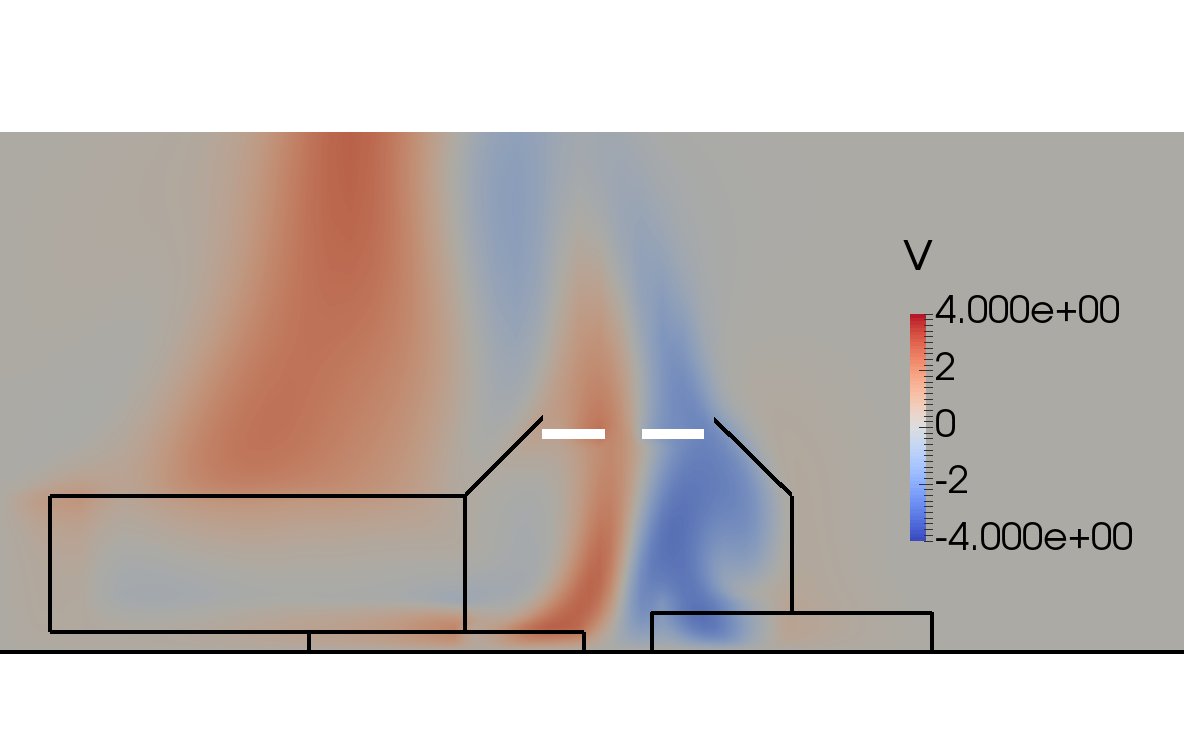
\includegraphics[width=.47\linewidth]{figs/v_field_vert}
  \label{fig:field_vert}
 \caption{Vertical slices through the middle of the vanes for the
 2016 Field Test. The top left is the streamwise velocity component
 (u), and the top right the vertical velocity, w. The bottom row shows
 the same plane, but now for the temperature field and azimuthal
 velocity. The turbine region is depicted at the top of the vanes as a
 white disk region.} 
\end{figure}

\begin{figure}[!htb]
  \centering
  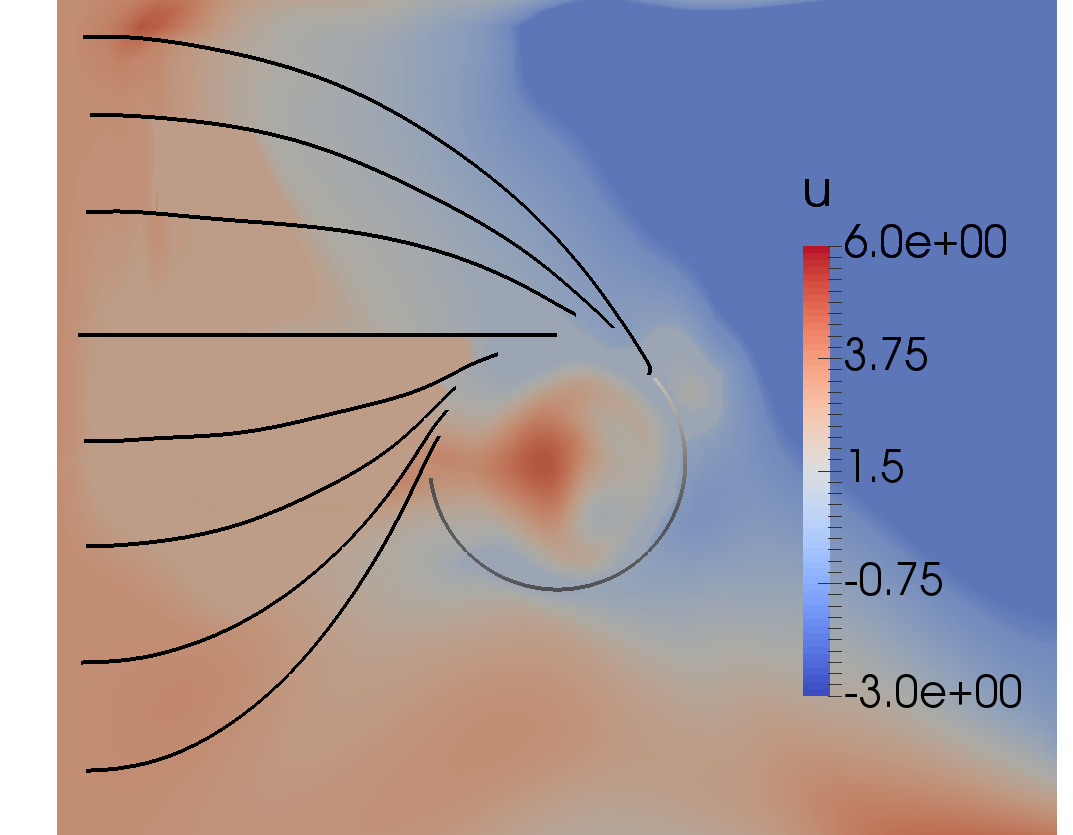
\includegraphics[width=.45\linewidth]{figs/u_field_hor}
  \hfill
  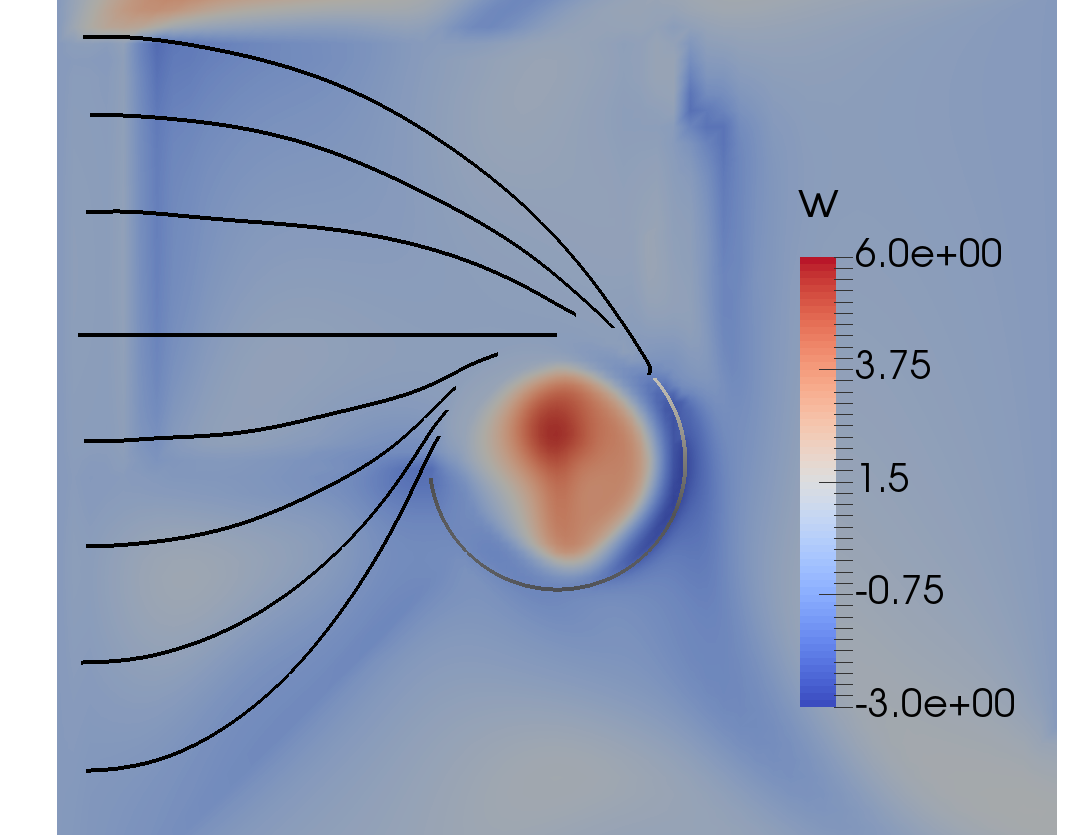
\includegraphics[width=.45\linewidth]{figs/w_field_hor}
  \\
  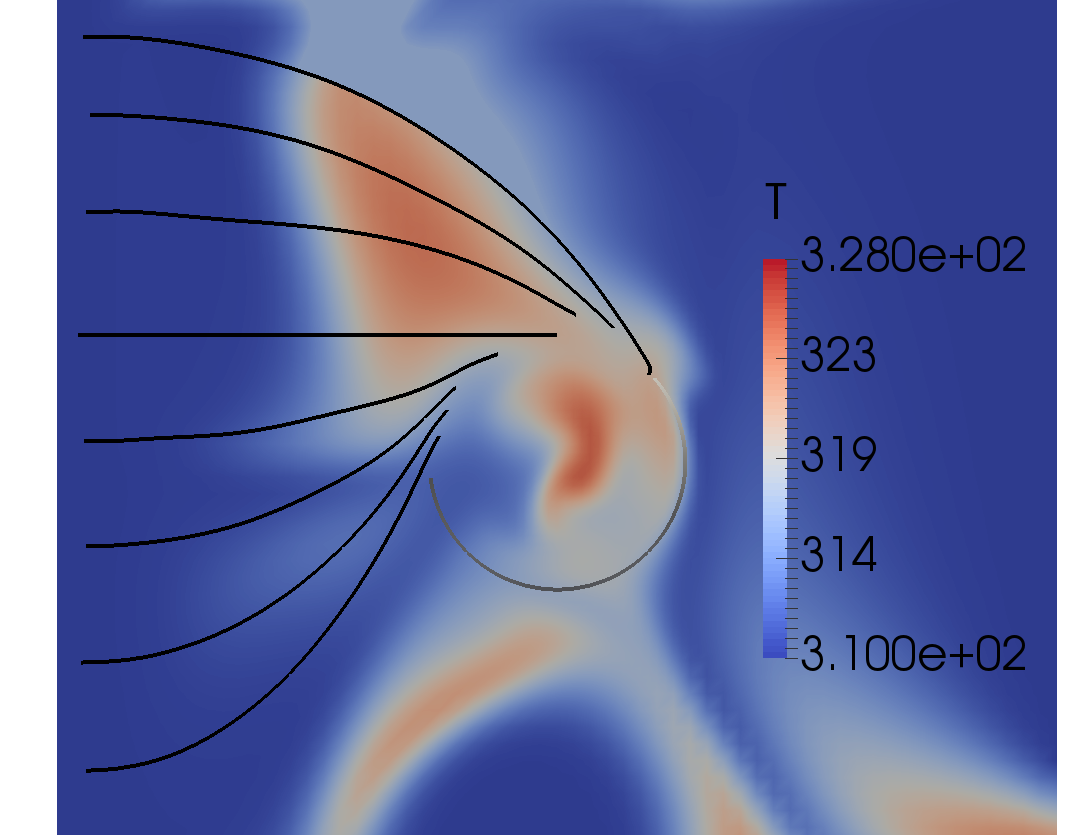
\includegraphics[width=.45\linewidth]{figs/T_field_hor}
  \hfill
  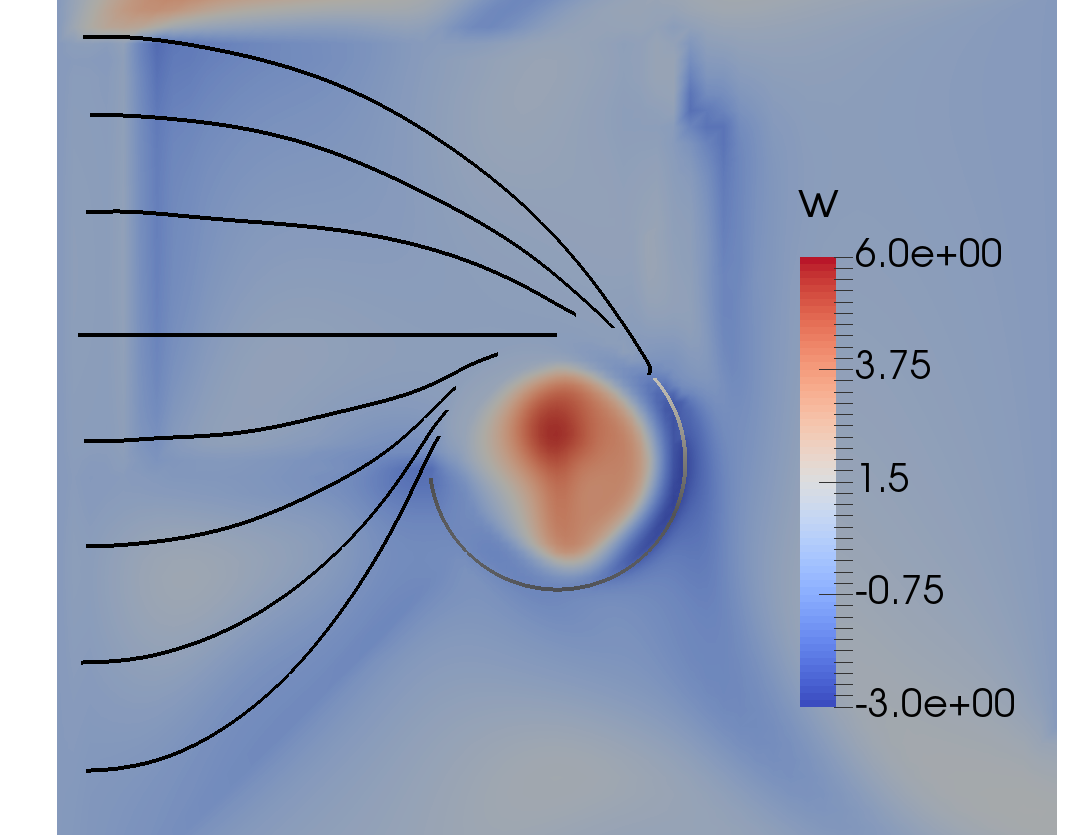
\includegraphics[width=.45\linewidth]{figs/w_field_hor}
  \label{fig:field_hor}
 \caption{Horizontal slices through the top of the vanes for the
 2016 Field Test. The top left is the streamwise velocity component
 (u), and the top right the vertical velocity, w. The bottom row shows
 the same plane, but now for the temperature field and azimuthal velocity.} 
\end{figure}

The velocity and temperature fields resulting from the 2016 field test 
simulations are shown in Figures~\ref{fig:field_hor} and
~\ref{fig:field_vert}, below. Generally speaking, the fields have
complicated, non-trivial structure. The majority of the flow is driven
into the vanes by the ambient upstream winds, where it accelerates due
to the contraction of the vanes towards the center of the SoV.
The vertical slices in Figure~\ref{fig:field_vert} clearly depict a
strong vertical velocity in the center of the device. This vertical
plume coincides with a coherent, high temperature ``thermal plume'', as
well as a region of intense rotation and azimuthal velocity. This flow
is driven upward where it flows past the turbine and out of the top of
the device. 

From the horizontal viewpoint shown in Figure~\ref{fig:field_hor}, it is
clear that the streamwise velocity has a complicated structure. The
vertical velocity is largely a circular plume that has expanded to fill
the cylindrical inner region of the turbine vanes. Unlike in the
thermal-only cases, no downward flow exists, and there is no formation
of a two-celled vortex. 

\begin{figure}
  \centering
  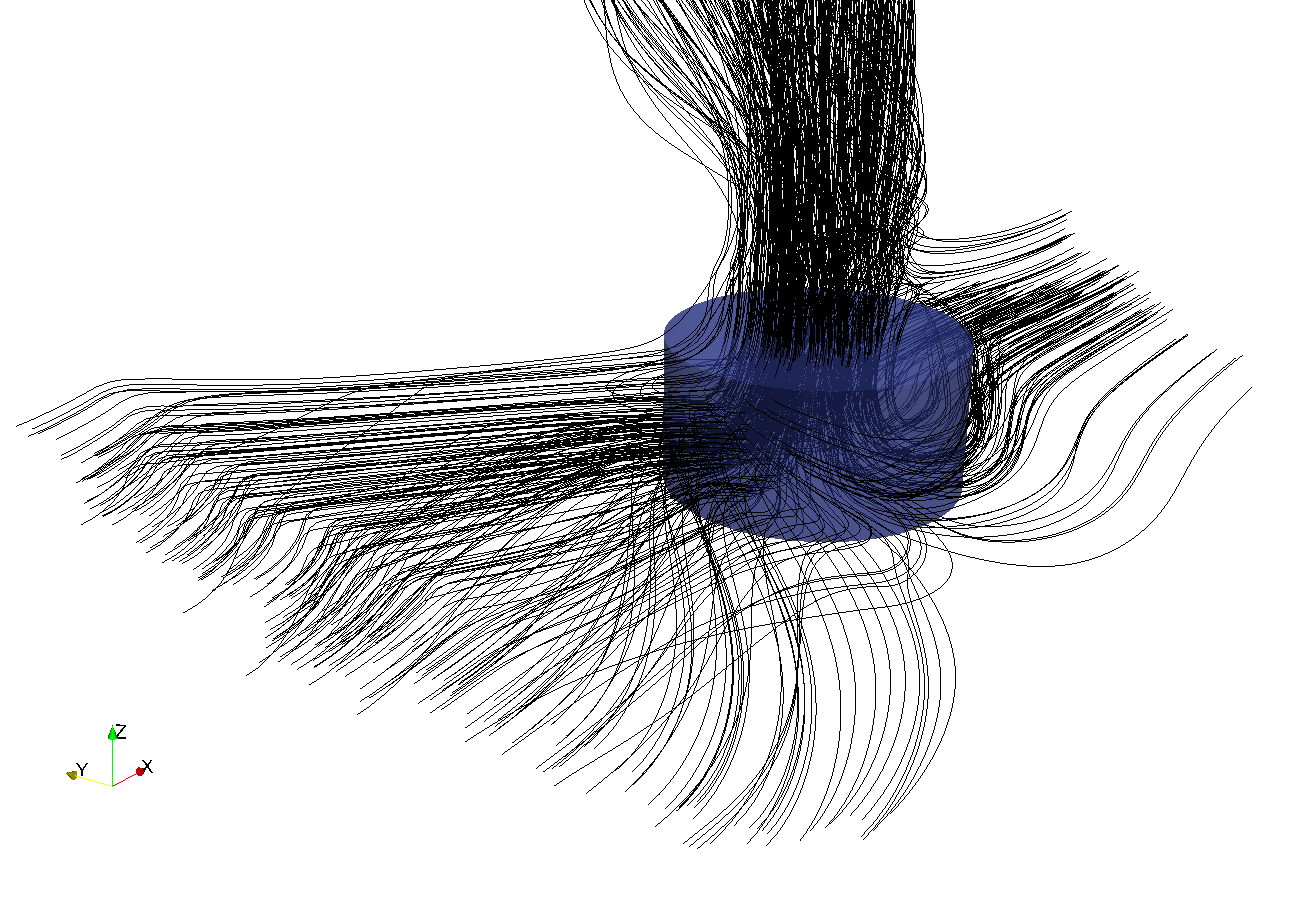
\includegraphics[width=.7\linewidth]{figs/field_streamlines}
  \label{fig:field_stream}
 \caption{Fluid entrainment through and around the apparatus. This was
 drawn by seeding particles into the flowfield and then advancing them  
 using an RK4 time integrator. An outline of the inner enclosure region 
 is shown to provide a sense of scale. The bottom left corner is the
 upwind direction. While a majority of the flow is coming from upstream
 of the device, a substantial portion of the flow is nevertheless
 entrained from the leeward side of the SoV. }  
\end{figure}

Figure~\ref{fig:field_stream} shows tracing particles advanced forward
and backward in time from the center of the device. This clearly shows
that the flow is drawn in from both the front and back of the SoV, and
that the device is entraining air from a region far larger than the SoV
vane diameter.  While a majority of the flow is coming from upstream of
the device, a substantial portion of the flow is nevertheless  entrained
from the leeward side of the SoV. Most of the entrained flow from
downstream of the vanes appears to be constrained come from the wake of
the SoV. It is also interesting to note that most of the backflow from
downwind side occurs very near the surface. While most of the radial
inflow to the SoV is from the downside side is near the surface, the
vortex is strong enough to entrain flow from outside the vanes above the
device.  

The 2016 field configuration has 4.77 kW of kinetic energy flux through
the top of the vanes, taken from a plane just below the turbine, which
is 608\% higher kinetic energy flux than the peak measurement produced in
the August 2015 Field test.  

\subsection{Sources of Error}
\label{sec:field_error}
%
%behaves like wind tunnel contraction
While these results are promising, there are several significant
shortcomings to these models and scenario conditions that substantially
impact the SoV performance. 

A major uncertainty is the opacity of the device. Ideally, the device
would be completely transparent. However, previous field tests
found that the SoV device shaded the inner region, which resulted in a
lower temperature inside the device than 
outside. As the physical trigger for the SoV is thermal buoyancy, this
greatly reduces the velocities inside the device, and so the kinetic
energy flux and power extracted by the turbine. For instance,
simulations performed with the ground temperature inside the vane region
set to the ambient air temperature (an admittedly ``worst-case
scenario'') found that the energy extracted by the turbine was reduced
to only 800 Watts. Thus, consistent with the results shown in
Section~\ref{sec:wind_impact}, the absence of a thermal to drive the
flow reduces the available kinetic energy flux (and thus, the power
extracted by the turbine) by more than half. 

%Scenario Uncertainty!!!!!!!!!!!

%Actuator disk under-estimates drag

%no model for drag on vanes (was reported by team)

%wind heading adjustments and measurements of flux reduction

No dynamics in the wind were considered, only a steady, mean wind
velocity. It may well be that even in the "thermal only" cases there
could be significant, zero mean wind fluctuations contributing energy. 
However, crude sensitivity analyses were performed by
adjusting the mean velocity of the wind by  $\pm 1 \text{m}/\text{s}$,
which indicated that the power generated by the turbine only increases
with higher wind velocity, and that most of the vortex structure and
character of the solution discussed in
Section~\ref{subsec:field_predict} remains valid, with only modestly
reduced velocities. 

%It is also possible that a substantial transient may exist during which
%the SoV 

A June field test in 2016 reported only modest velocities through the
prototype apparatus.
While substantial, the uncertainties describe above are not sufficient
to account for the weakness of the observed flow, indicating a
potentially significant model error that had not previously been
considered. The subsequent sections detail two possible modeling
errors that were investigated in detail, and may account
for the significantly reduced flow observed in the field. 

\section{Turning Vane Drag}

The first model correction proposed is to introduce drag along the
turning vanes to account for the skin friction along the surface. To
introduce a force of parasitic drag, the turning vane forcing 
representation described in Section~\ref{subsec:vane} need only be
modified to introduce an additional force that acts in opposition of the
fluid velocity. Thus, in addition to forcing the flow to align with the
vane surface, the flow will also be slowed. The vane formulation now
acts in a dissipative manner, and is not energy conserving. 

Our unit forcing vector ${\bf \hat f}$ is simply the negative normalized inner
product of the velocity, ${\bf u}$, and the turning vane tangent vector
${\bf \hat t^v}$,  
\begin{equation}
- \frac{{\bf u} \cdot {\bf \hat t^v}}{|| {\bf u} \cdot {\bf \hat t^v}
 ||} = {\bf \hat f}.  
\end{equation}
The volumetric force applied is, 
\begin{equation}
 F = {\bf \hat f} \, C_f \, \frac{1}{2} \frac{\rho || {\bf u} ||^2}{\delta}
\end{equation}
Where $C_f$ is the skin friction coefficient (which must be determined),
$\rho $ is the density and $\delta$ the channel half width. 
For $C_f$, we use Dean's Correlation\cite{johnson1998handbook}, 

%ane
%
%https://books.google.com/books?id=JBTlucgGdegC&pg=SA13-PA51&lpg=SA13-PA51&dq=dean%27s+correlation+fluids&source=bl&ots=auW8XopUC9&sig=DDxuQONFvqly5KQOocSPr39rS70&hl=en&sa=X&ved=0ahUKEwii3vX9wZHOAhXmxYMKHUqlChYQ6AEIJTAB#v=onepage&q=dean%27s%20correlation%20fluids&f=false 
%
\begin{equation}
 C_f = 0.073 \, (Re)^{-0.25}. 
\end{equation}
Where the Reynolds number is defined as, 
\begin{equation}
 Re = \frac{u\, \delta}{\nu}.
\end{equation}

Some roughness elements exist across the vanes. In addition to
non-smooth surface materials, the design of the field test apparatus
ultimately relied upon posts to hold the turning vanes. These posts were
pieces of wood which were modeled as roughness elements. In order to
determine $C_f$ for these cases, the Colebrook formula\cite{Colebrook367},
% Colebrook, C. F.; White, C. M. (3 August 1937). "Experiments with
% Fluid Friction in Roughened Pipes". Proceedings of the Royal Society
% of London. Series A, Mathematical and Physical Sciences. 161 (906):
% 367–381. doi:10.1098/rspa.1937.0150 
was used to provide an estimate for the friction factor given a
roughness height, $\epsilon/D$,  
\begin{equation}
 \frac{1}{\sqrt{f}} = -2.0 \text{ log}\left(\frac{\epsilon/D}{3.7} + \frac{2.51}{Re\sqrt(f)}\right).
\end{equation}
 With the assumption that for large roughness the Reynolds number term
 contribution is not significant, the function is no longer implicit in
 $f$ and can be determined directly, 
\begin{equation}
 f = \left(2.0 \text{ log}\left(\frac{\epsilon/D}{3.7}\right)\right)^2. 
\end{equation}
%Then, a Moody chart was consulted to provide the the 
Note that D here is the hydraulic diameter which must account for the
two plates (we treat the vanes as a channel),
\begin{equation}
D_H = \frac{4 A}{P} = \frac{4 (2w)\delta}{2w} = 4 \delta
\end{equation}
Where $\delta$ is the channel half width, or in our case, the distance
between the vanes. To construct a ``worst-case'' scenario, we consider
the smallest distance between the vanes, which occurs near the center of
the SoV. Furthermore, we consider roughness heights based on a
two-by-four (which were used as supports for the
vanes). Even for this worst case scenario, the velocities on the vanes
are not substantially reduced with the addition of the drag model. The
flow field kinetic energy flux was never reduced more than 12\%. 
This crude model indicates that the reduced flows observed during the
June 2016 field tests are not attributable to skin friction drag on the
turning vanes.  


\section{Blade Solidity Modification}
\label{sec:solidity}
%
%https://en.wikipedia.org/wiki/Blade_solidity
%
It was noted that wind turbines typically possess three blades, versus
the eight blades used in the 2016 field test. This is therefore a
substantially increased turbine solidity versus common engineering
designs. It is expected that we are operating in a regime not common to
typical actuator disk models. 

The power output of a turbine is proportional to the thrust that it
exerts onto the flow, and the larger the thrust, the larger the flow
resistance the turbine presents to the flow. The maximum power for any
wind turbine must lie in between two extremes, i.e. high and
a low impedance both result in minimal power
extraction\cite{solidity_oxford}.  

For the case of high impedance, little fluid flows through the
turbine and instead flows around the device. This gives the appearance of
the turbine being ``blocked''. In the case of low impedance, the turbine
hardly affects the flow, and less power is extracted than could be. 

Thus, an ``efficient'' impedance to the flow is one that strikes the 
right balance between solidity and tip speed ratio. If the solidity is
high, the operating tip speed ratio must be lower to avoid too high an
impedance. 

However, it is hard to predict the precise effects of the various
phenomena, which is why it is difficult to comment on the overall
performance of a particular machine in a specific
scenario. %Turbine design is highly specialized for 

However, the actuator disk model treats the flow in the disk region as
if it was flowing through a rotor with identical solidity but an
infinite number of blades. A model correction was introduced that
attempts to represent the fact that as the number of turbine blades
increases, the pressure across the actuator disk should rise. This is
accomplished by adjusting the area of the actuator disk down by the
ratio of the free area in the disk versus the blade sizes. 

%A second model correction was therefore introduced with the aim of attempting to
%discern if the turbine 


% too high an impedance
%This has several important implications.  

%A low tip speed ratio implies increased torque, requiring a larger
%and higher cost gearbox. In addition, the lower the tip speed ratio, the
%higher the maximum angle of attack, which can be problematic with regard
%to blade stalling. 

%
% howevr, it is hard
%

%When applied to a rotor with a finite number of blades, 


The length of each blade blocking vertical flow in the actuator disk is, 
\begin{equation}
  c * \text{Cos}(\beta(r)) = c_x(r). 
\end{equation}
The total length in an annular region that is blocking is therefore,
\begin{equation}
  N * c_x(r) = l_B(r),
\end{equation}
Where N is the number of blades. 
Then, the ratio of an annular length that is impeded by blades is, 
\begin{eqnarray}
 B(r) =& \frac{2\pi r- l_B(r)}{2 \pi r}\\
 B(r) =& 1- \frac{l_B(r)}{2 \pi r}. 
\end{eqnarray}
Note that a ``floor'' function is needed to ensure the solidity ratio
does not go below zero. 

For a 1D control volume analysis for the region, the continuity
equation is, 
\begin{eqnarray}
 \rho V_z' A' =& \rho V_z A,\\
 V_z' =& V_z \frac{A}{A'}, \\
 V_z' =& \frac{V_z}{B(r)}.
\end{eqnarray}
This implies that $V_z' \rightarrow \infty$ as $A' \rightarrow
0$. This is as expected, as the blockage becomes more severe, the flow
would need to move at greater speed to go through it. 

The flow angle with respect to turbine velocity is therefore modified 
from Equation~\ref{eq:fan_direction} in
Section~\ref{sec:actuator_disk},
\begin{equation}
 \theta_f = \text{tan}^{-1}(\frac{{\bf u_{\text{up}}}}{{\bf u_{\text{fwd}}}})
\end{equation}
to,
\begin{equation}
 \theta_f = \text{tan}^{-1}(\frac{{\bf u_{\text{up}}}}{B(r) {\bf  u_{\text{fwd}}}}). 
\end{equation}
As $B(r) \rightarrow 0$, $\theta_f \rightarrow \pi$, e.g. 90 degrees. In
this way the velocity vector will be completely aligned with drag. 

Furthermore Equation~\ref{eq:force_turb}, 
\begin{equation}
 F = \frac{1}{2}\frac{c \rho U_p^2}{A}(C_L \cdot {\bf n_{\text{lift}}} + C_d
  \cdot {\bf n_{\text{drag}}})
\end{equation}
is modified so that, 
\begin{equation}
 \bar U_p^{2} = \left(\frac{U_p}{B(r)}\right)^2
\end{equation}

This turbine modification for solidity has a significant impact on the
power extracted by the turbine. A comparison between the number of
turbine blades and the power generated by the turbine for both the
baseline turbine and the turbine with the solidity modification is shown in
Figure~\ref{fig:turbine_solidity}. The results are quite consistent with
two blades, show a notable inconsistency at four blades, and completely
diverge at higher blade count. 
%Only even number of blades were
%considered due to the expectation that 

  \begin{figure}[!htb]
   \begin{center}
    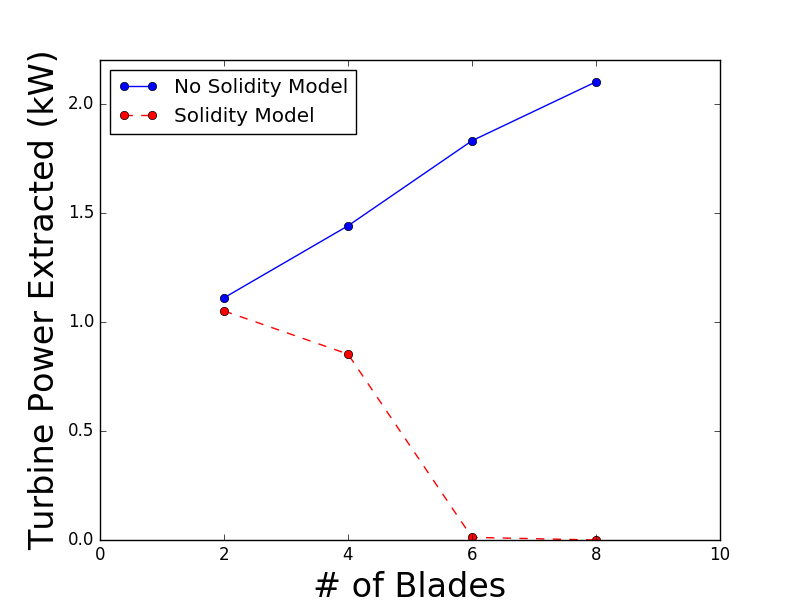
\includegraphics[width = 10 cm]{figs/solidity}
    \caption{The power extracted by the turbine as a function of blade
    count. The blue straight line indicates the turbine model as defined
    in Section~\ref{sec:actuator_disk}, and the red dashed line
    indicates the power output of the turbine after the solidity
    modification.}
    \label{fig:turbine_solidity}
   \end{center}
  \end{figure}

This model modification indicates that the prior prediction of eight
turbine blades in Section~\ref{sec:turb_design} was too large. Instead,
a turbine with substantially reduced solidity is preferred. Based on
Figure~\ref{fig:turbine_solidity}, a turbine with similar
characteristics in terms of length, location and twist but reduced from
eight blades to four or two blades is expected to mitigate the
substantially reduced performance observed in the field. 

This crude model is admittedly extreme, as it effectively models the
blades as flat plate bluff bodies, with the flow completely
separated on the leeward side. Ideally, the flow should be smoothly
turning through the blading, and not separate. Thus, it is possible that
this estimate is overly pessimistic. Regardless, this is the only model
correction that was explored that is plausibly capable of explaining the
2016 field observations noted in Section~\ref{sec:field_error}. 

Interesting enough, there have been actuator disk models used with wind
turbines that indicate operating at low tip speed ratios with high
solidity ratios would possess power coefficients close to Betz-like
limits of efficiency\cite{WE:WE118}. It is therefore possible that the
actuator disk model is generally unsuited for high solidity regimes, and
that the correction presented here is more generally useful. 

%todo\todo{what about shading?}

\section{Estimating the Upper Limit on Power Extraction}
\label{sec:peak_estimate}

All of the results in Section~\ref{subsec:field_predict} were
generated\todo{bf this section!}
using $90^{\circ}$ semicircle blade geometries, as shown in Figure
\ref{fig:90_drag}. The only other blade geometries considered were the
flat plate and $180^{\circ}$ arcs, which were universally found to be
inferior. Time constraints required fabrication of the turbine in short
order, and a limited budget encouraged inexpensive (and therefore
simple) turbine blades. Finally, the design space was limited to
readily available drag polar data due to the expense and difficulty of 
fabricating non-standard turbine blades. Risk mitigation also played a
role, with an emphasis on traditional, and therefore well-vetted turbine
blade design. %While several comparisons have been performed with
%different choices of turbine blades (flat plate, 180 degree semicircles,
%etc. ) this was not an exhaustive survey. 
%Nevertheless, this is not an exhaustive exploration of turbine
%blade design, and the question remains, ``Could more power be extracted
%with a different rotor geometry?''. 
This section details an additional computational research program
performed after the turbine fabrication with the intent of estimating
the upper limit of power extraction with an idealized turbine. 

Practical utility-scale wind turbines achieve at peak 75\% to 80\% of
the Betz limit\cite{burton2001wind}. The Betz-limit states a theoretical
maximum of 59\% of the wind's power may be captured. Therefore,
practical wind turbines extract less than half of the available kinetic
energy flux. 
Comparing the kinetic energy flux of simulations without the turbine to
the power extracted by the turbine, we note that our simulations
typically predict power extraction ratios slightly less than fifty
percent, indicating that our efforts are not significantly better or
worse than could be expected. While this provides an estimate, the
Betz-limit is likely not accurate for this case. Any analysis of the
power that can be extracted is complicated by the presence of
considerable vertical and azimuthal flow in the vortex, and so the
design considerations are different from those for a classical wind
turbine.  

The objective then, is to formulate a more generalized approach to the
turbine vane parameters to permit an optimization that is not
constrained to a particular turbine blade geometry. Rather, this
approach seeks to estimate the upper limit of power extracted. The
rationale behind this is to provide an upper bound on the power that can 
be extracted for a particular configuration, which can then be used as
input for feasibility considerations of the SoV.  

It is desirable to perform these estimates within the context of the
actuator disk model (see Section~\ref{sec:actuator_disk}). While
actuator disk models are commonly
optimized\cite{790585,WE:WE487,en5093425,adkins1983design}, the lift and 
drag polars are not parameters that are varied in these schemes. Rather,
a given blade geometry is assumed and then the rotation rate, blade
angle and chord length (for instance) are optimized.   

Conversely, airfoil optimization is a rich field with sophisticated and
well-vetted
techniques~\cite{drela1998pros,lewis2001aerodynamic,Chehouri2015361},
but these methods do not use an actuator disk model, and focus on the
shape optimization of the airfoil geometry (and through this, the lift
and drag polars).  

To address the possibility of further turbine blade
improvements, while continuing to use an abstract actuator disk model,
%while simultaneously not representing the blade geometry
%proper
this section details a formulation for a generic set of drag 
polars. These generalized drag polars permit exploration of a broader
design space. The optimization of this model can be fully coupled to the
flow, and so does not violate any Betz-like considerations that might
similarly arise in an analysis of frozen flow fields.
The drag polars are selected to be generic functions and are optimized to
maximize the power extracted by the rotor. While the resulting drag
polars might not be physically  realizable, they represent a ``best
case'' upper bound indicating the peak power that might be extracted
with further rotor design iterations. This ``limiting case'' is useful
for evaluating the system feasibility from a technological standpoint,
by providing the peak power that could be extracted for a given vane
geometry. 

The power extracted by the turbine is, \todo{flip to Bc, as in other chapter}
\begin{equation}
 P = \Omega \, Q
\end{equation}
where the torque, Q, is\cite{morgado2014validation}, 
\begin{equation}
 Q = A_R \int_0^{2\pi} \int_{r_{\text{min}}}^{r_{\text{max}}} F''_{\tau}\, r\, dr d\theta.
\end{equation}
Here, $A_R$ is the relative area coefficient which is, 
\begin{equation}
A_R = \frac{c B (r_{\text{max}}-r_{\text{min}})}{\pi(r_{\text{max}}^2-r_{\text{min}}^2)}
\end{equation}
where B is the number of blades, $r_{\text{max}}$ and $r_{\text{min}}$
are the turbine radii, and $F''_{\tau}$ is the force per unit
area on the turbine, which is, 
\begin{equation}
 F''_{\tau} = \frac{F_{\tau}}{cl}= \frac{1}{2}\rho U_R^2 \, C_{\tau}.
\end{equation}
with $U_R$ the magnitude of relative velocity and $c$ is the blade chord
length, which is assumed to be constant (not a function of the radius,
for instance). Finally, $C_{\tau}$ is the tangential force coefficient,
which depends on the local lift and drag coefficients, and the
flow angle, $\phi$, 
\begin{equation}
 C_{\tau} = C_L \,\text{sin}(\phi) + C_D \,\text{cos}(\phi)
\end{equation}
Combining the equations above results in an expression for the power
that explicitly depends on the lift and drag coefficients, 
\begin{equation*}
 P = \frac{\Omega \rho c B (r_{\text{max}}-r_{\text{min}})}{2 \pi(r_{\text{max}}^2-r_{\text{min}}^2)}
\int_0^{2\pi}
\int_{r_{\text{min}}}^{r_{\text{max}}} U_R(r,\theta,\Omega)^2 \left(C_L
						     \,\text{sin}(\phi)
						     + C_D
						     \,\text{cos}(\phi)
						    \right) r\,dr d\theta. 
\end{equation*}
We lump the constant terms together, 
\begin{equation}
E_{\tau} = \frac{\Omega \rho c B (r_{\text{max}}-r_{\text{min}})}{2
 \pi(r_{\text{max}}^2-r_{\text{min}}^2)}
\end{equation}
 and separate this equation, 
\begin{align}
 P_L = E_\tau
 \int_0^{2\pi}
  \int_{r_{\text{min}}}^{r_{\text{max}}} U_R(r,\theta,\Omega)^2 \, C_L(\phi,r)
 \,\text{sin}(\phi)\, r\,dr d\theta,  \label{lift} \\
 P_D = E_\tau
 \int_0^{2\pi}
  \int_{r_{\text{min}}}^{r_{\text{max}}} U_R(r,\theta,\Omega)^2 \, C_D(\phi,r) \,\text{cos}(\phi)\, r\,dr d\theta. \label{drag}
\end{align}
Note that we have assumed $C_D = C_D(\phi,r)$ and $C_L = C_L(\phi,r)$,
namely, that the coefficients vary with the flow direction and may vary
radially, due to twisting the blade angle. Furthermore, the flow
direction, $\phi$, varies with the location and the blade speed,
in that $\phi=\phi(r,\theta,\Omega)$. The relative velocity is the
quantity, $U_R = U - U_\tau$, e.g. the difference in velocity between
the turbine and the flow. The turbine has no axial velocity ($w_\tau =
0$) and a constant rotation speed, and so the two components of velocity
in the plane of rotation can be expressed as,
\begin{align}
 u_\tau = \Omega \,r\, \text{sin}(\theta)\\
 v_\tau = \Omega \,r\, \text{cos}(\theta)
\end{align}

Our objective is now to discover what these unknown functions of lift
and drag are. To do this, we specify an optimization problem such that, 
\begin{equation*} 
 \text{Max } P(C_L,C_D) \quad \text{ subject to: }
  \begin{cases}
   |C_L| < C_L^{\text{Max}}, \\
   0 < C_D < C_D^{\text{Max}}. \\
  \end{cases}
\end{equation*}

In words, the drag must be specified to be greater than zero, but
the lift can be negative. This is a problem in the calculus of
variations, where the objective is to maximize a
functional subject to imposed
constraints~\cite{thornton2004classical,bradbury1968theoretical,2015JFM...784..565S}.   

%
% does this argument still work?!?
%
The integral shown in Equation \ref{lift} above can be bounded by 
Schwarz's inequality,  
\begin{align*}
  \left[
    \int_0^{2\pi}
    \int_{r_{\text{min}}}^{r_{\text{max}}} C_L(\phi,r)\, U_R(r,\theta,\Omega)^2
 \,\text{sin}(\phi)\, r\,dr d\theta \right]^2 \le \\
  \int_0^{2\pi} \int_{r_{\text{min}}}^{r_{\text{max}}} C_L^2(\phi,r) dr d\theta\,
  \int_0^{2\pi} \int_{r_{\text{min}}}^{r_{\text{max}}} U_R(r,\theta,\Omega)^4 
 \,\text{sin}^2(\phi)\, r^2\,dr d\theta.
\end{align*}

In this way the first integral quantity,
\begin{equation}
  \int_0^{2\pi}
 \int_{r_{\text{min}}}^{r_{\text{max}}} C_L^2(\phi,r) dr d\theta, 
\end{equation}
is clearly maximized when $C_L(\phi,r) = C_L^{\text{max}}$. 
The result for Equation \ref{drag} is identical. Now, for these
conditions, we are interested in largest attainable values. For the drag
coefficient, $C_D^{\text{Max}}$ is two. % refmunson 
This corresponds to a flat plate perpendicular to the flow.
The lift coefficient peak is about 1.75. This design is not necessarily
physically realizable, but represents an absolute maximum. 

Therefore, our lift/drag functions may be expressed as,
\begin{align*} 
 C_D(\phi) = \bar C_D \, \psi(\phi) 
  \begin{cases}
   \psi(\phi) = 1 \text{ if sin}(\phi) > 0,   \\
   0 \text{ else} \\
  \end{cases} \\
 C_L(\phi) = \bar C_L \, \Psi(\phi) 
  \begin{cases}
   \Psi(\phi) = 1 \text{ if cos}(\phi) > 0,   \\
   -1 \text{ else}. \\
  \end{cases}
\end{align*}
Where $\bar C_L = 1.7$ and $\bar C_D = 2.0$. The plot of these drag
polars are shown in Figure \ref{drags}. 

\begin{figure}[!htb]
  \begin{center}
    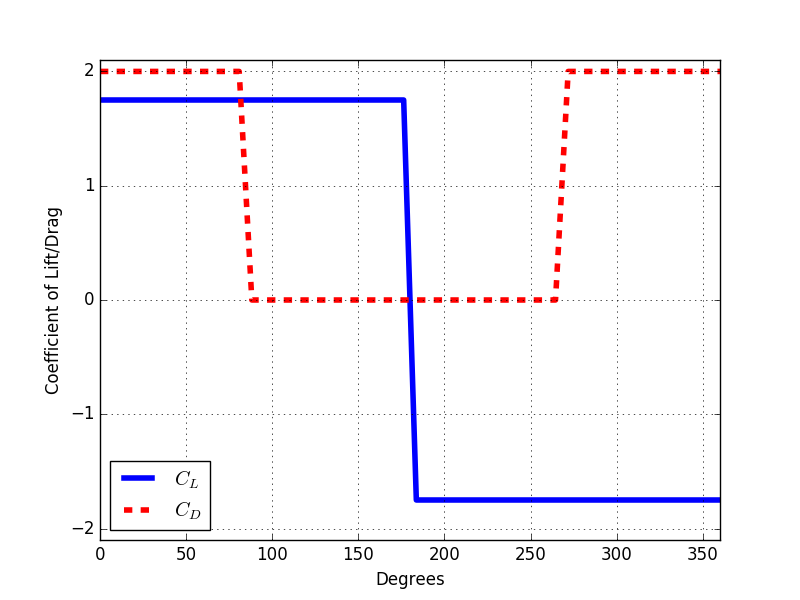
\includegraphics[width = 12 cm]{figs/opt_drags}
    \caption{The uncalibrated idealized drag polars.} 
    \label{drags}
  \end{center}
\end{figure}

%Thus, the drag polars
%have the form, 
%\begin{align*} 
% &C_L(\phi) = 
%  \begin{cases}
%    1.75& \quad 0^{\circ} \le \phi \le 180^{\circ}, \\
%   -1.75& \quad 180^{\circ} \le \phi \le 360^{\circ}.  \\
%  \end{cases}\\
% &C_D(\phi) = 
%  \begin{cases}
%    2.0& \quad -90^{\circ} \le \phi \le 90^{\circ}, \\
%      0& \quad 90^{\circ} \le \phi \le 270^{\circ}.  \\
%  \end{cases}\\
%\end{align*}

Under this approach, the turbine extracts so much energy from the flow
that the vortex loses its coherence and the power extracted becomes
negative (e.g. the constant velocity turbine is adding energy to the
flow). %\todo{add image}
This implies a limit on how much of the energy can be extracted before
disrupting the flow so greatly that the vortex cannot be maintained.   
Consistent with the results from Section~\ref{sec:field_error},
the vortex is not robust, and the feedback from extracting more power
from it (manifest as increased blade solidity) causes a collapse of the
vortex structure. It is interesting to note that the vortex collapse is
not subtle, with the power extracted discontinuously dropping to zero or
negative values. 

To withdraw from the vortex disruption point, the drag
polars are calibrated by reducing $\bar C_L $ and $\bar C_D$ so that the 
vortex does not dissipate and the power extracted remains positive. The
parameters were adjusted by hand, so the calibration is crude. The
optimal parameters found were $\bar C_L = 1.1$ and $\bar C_D = 1.5$. It
is interesting to note that this is nearly the average of the drag
polars shown in Figures~\ref{fig:flat_plate_drag},~\ref{fig:semi_drag}, 
and\ref{fig:90_drag}. The solution flow in the case of the idealized
turbine remains similar to the results shown in
Section~\ref{subsec:field_predict}, and so are not depicted here. 

The steady state power extracted by the ideal turbine 
increased from the previous best attained with the 90 degree
semicircles, to 2.76 kW. It is interesting to note that this is 58\% of
the available kinetic energy flux measured just upstream of the turbine,
indicating that the turbine is very close to the Betz-limit of
59.3\%. While as indicated previously, the Betz-limit is likely to be
inaccurate for rotating flows, it is nevertheless interesting that the
idealized turbine would extract power so close to the maximum predicted by
Betz.  This provides a weak limit (even under these idealized
conditions) bounding the power that can be derived from this
flow. Furthermore, this indicates that previous estimates of the power
that might be extracted from the flow are not greatly limited by the
present turbine design. This is an important element of the system
feasibility assessment, as it provides evidence against the turbine
being a source of considerable inefficiency.  

%discredits any 

% as it implies that any assessments of the system feasibility 
